\documentclass[11pt,a4paper]{article}
\usepackage[utf8]{inputenc}
\usepackage[T1]{fontenc}
\usepackage{lmodern}
\usepackage{geometry}
\geometry{margin=1in}
\usepackage{graphicx}
\usepackage{booktabs}
\usepackage{tabularx}
\usepackage{hyperref}
\usepackage{titlesec}
\usepackage{float}
\usepackage{xcolor}
\usepackage{amsmath}

\hypersetup{
    colorlinks=true,
    linkcolor=blue,
    filecolor=magenta,      
    urlcolor=cyan,
    pdftitle={Toxin Circuits in ESM-2},
    pdfpagemode=FullScreen,
}

\title{\textbf{Toxin Circuits in ESM-2: Mechanistic Interpretability Reveals Why Structure-Aware Probes Resist ProteinMPNN Redesign}}
\author{\textbf{AiXbio Research} \\ \textit{Submitted to AIxBio Hackathon 2026}}
\date{\today}

\begin{document}

\maketitle

% ============================================================
% ABSTRACT
% ============================================================
\begin{abstract}
Standard biosecurity screening flags dangerous protein sequences by sequence identity (BLAST).
We show that ProteinMPNN redesigns toxin sequences below every BLAST threshold---achieving
0\% BLAST detection---while a linear ESM-2 probe maintains 93.9\% detection with no retraining.
Using interPLM Sparse Autoencoders (SAEs), we identify 50 of 10,240 features explaining probe
performance at 205$\times$ compression. These features are \textit{amplified}, not suppressed,
by redesign (mean transfer ratio = 1.28): ProteinMPNN preserves structural fold topology, and
fold topology is precisely what the circuit encodes. We characterise the adversarial robustness
spectrum through four attacks---ProteinMPNN blackbox (6.1\% evasion), HotFlip gradient-guided
sequence attack (100\%), and embedding-space attacks (100\%)---demonstrating the security
boundary lies at gradient access, not sequence vs.\ embedding space. Direct Probe Attribution
identifies layer 32 as the circuit bottleneck. A Universal Adversarial Perturbation achieves
100\% evasion at $\epsilon=1.0$ (security margin $\epsilon=0.5$) via a stable direction
at $-0.805$ cosine with the probe---revealing manifold geometry, not probe weakness.
Zero-shot scanning of 1,000 UniRef50 sequences discovers 248 candidates enriched 4.75$\times$
for secreted signal peptides, including a Hemolysin (0.9996), Leukotoxin (0.9922), and the
confirmed fungal effector Ecp2 (0.9905) from \textit{Colletotrichum}---cross-kingdom
generalisation from a probe trained exclusively on animal and bacterial toxins.
Furthermore, we show that Sparse Autoencoders (SAEs) can mathematically disentangle adversarial camouflage, recovering 38\% of "Double-Evaders" that fool both BLAST and dense linear probes. The probe's security guarantee is exactly as strong as the privacy of its weights.
\end{abstract}

% ============================================================
\section{Introduction}
% ============================================================

Dual-use protein screening relies on sequence-identity thresholds. Wittmann \textit{et al.}
(2025) demonstrated that ProteinMPNN, RFdiffusion, and EvoDiff can redesign toxin sequences
below standard 40\% identity thresholds, bypassing BLAST-based screening. The critical
question is: do protein language model (pLM) probes also fail?

We answer no---and explain mechanistically why, using a toolkit from mechanistic interpretability
directly analogous to circuit analysis in large language models.

\textbf{Contributions:}
\begin{enumerate}
    \item \textbf{Quantitative gap}: BLAST detects 0\% of ProteinMPNN redesigns; ESM-2 probe detects 93.9\%.
    \item \textbf{SAE circuit}: 50 sparse features (205$\times$ compression) explain the probe; mean transfer ratio 1.28 shows redesigns \textit{amplify} toxin features.
    \item \textbf{Attack taxonomy}: Four attacks spanning blackbox to oracle, with the security boundary at gradient access (not sequence/embedding space).
    \item \textbf{UAP geometry}: Universal attack direction stable at cos $= -0.805$ across all $\epsilon$---a structural property of the toxin manifold.
    \item \textbf{Zero-shot discovery}: 248 UniRef50 candidates including cross-kingdom detection of fungal effectors and WHO Priority 1 pathogen proteins.
    \item \textbf{Mutation robustness}: 0/1,179 single-point mutations evade detection; the circuit reads chemical polarity, not sequence identity.
\end{enumerate}

% ============================================================
\section{Methods}
% ============================================================

\subsection{Data}
\begin{itemize}
    \item \textbf{Natural toxins}: 1,712 sequences from UniProt (reviewed, toxin annotation), clustered at 30\% identity
    \item \textbf{Controls}: 2,072 non-toxic human proteins (matched length distribution)
    \item \textbf{Redesigns}: 100 toxin structures folded with ESMFold $\rightarrow$ ProteinMPNN (10 seq/structure) $\rightarrow$ 723 unique redesigns; all below 30\% identity to training toxins
    \item \textbf{UniRef50 scan}: 1,000 randomly sampled sequences (seed=42), scored zero-shot
\end{itemize}

\subsection{ESM-2 Probe}
Linear probe trained on mean-pooled ESM-2 650M embeddings at layer 33. Binary cross-entropy loss, Adam optimiser, 150 epochs.

\subsection{SAE Feature Analysis}
interPLM pre-trained SAEs (ESM-2-650M, layer 33, 10,240 features). Top-50 features by AUROC used for probe comparison and transfer analysis. Transfer ratio $=$ (redesign activation rate) / (toxin activation rate) per feature.

\subsection{Direct Probe Attribution (DPA)}
For a linear probe with weight vector $\mathbf{w}$ and ESM-2 residual stream decomposed as $\mathbf{h}_{33} = \sum_l \Delta\mathbf{h}_l$:
\begin{equation}
\text{DPA}_l = \mathbf{w} \cdot \text{mean\_pool}(\Delta\mathbf{h}_l)
\end{equation}
Exact because the probe is linear and ESM-2 is a residual network. Computed over 75 toxin/control/redesign pairs.

\subsection{Attention Head Ablation}
160 heads across 8 key layers (17--20, 29--32) ablated individually across 10 toxin sequences. DPA drop measured per head. Note: DPA drops are not additive across heads due to compensatory effects in non-linear layers; absolute values reflect disruption magnitude, not independent contribution.

\subsection{Adversarial Attack Taxonomy}
\begin{enumerate}
    \item \textbf{ProteinMPNN (blackbox)}: Structure-conditioned redesign; no access to ESM-2 or probe.
    \item \textbf{HotFlip (gradient-guided, sequence-space)}: Backpropagate through ESM-2 to compute first-order substitution scores; greedy substitution. Analogue of GCG \cite{zou2023universal}.
    \item \textbf{PGD (iterative, embedding-space)}: Projected gradient descent within $L_2$ $\epsilon$-ball \cite{madry2018pgd}.
    \item \textbf{pSSR / UAP (oracle, embedding-space)}: Gradient descent on embeddings with $L_2$ constraint; single universal vector optimised across all toxins simultaneously.
\end{enumerate}

\subsection{Universal Adversarial Perturbation (UAP)}
Single 1280-dimensional $\delta$ optimised via Adam (lr=0.1, 250 steps) to minimise probe scores across all toxin embeddings simultaneously, projected onto $L_2$ ball of radius $\epsilon$. Epsilon sweep: $\epsilon \in \{0.05, 0.1, 0.25, 0.5, 1.0, 1.5, 2.0, 3.0, 5.0\}$.

\subsection{Deep Mutational Scan (DMS)}
All 1,179 single-point mutants of a 62 aa toxin sequence embedded through ESM-2 layer 33 and scored. Conservative substitution analysis at position 29 (N29) across all 19 amino acid substitutions.

\subsection{Cross-Family Holdout}
Entire toxin families (neurotoxin, phospholipase, conotoxin, snake) held out one at a time; probe retrained on remaining families and evaluated on held-out family. Tests whether circuit generalises across toxin architectures.

\subsection{Zero-Shot UniRef50 Scan}
1,000 randomly sampled UniRef50 sequences scored through the trained probe. Candidates scoring $> 0.85$ annotated via UniProt REST API. Signal peptide enrichment tested by Fisher's exact test.

% ============================================================
\section{Results}
% ============================================================

\subsection{Layer Sweep --- Layer 33 Is Best}

\begin{table}[H]
\centering
\begin{tabular}{cc}
\toprule
\textbf{Layer} & \textbf{AUROC} \\
\midrule
1 & 0.9678 \\ 9 & 0.9881 \\ 18 & 0.9842 \\
24 & 0.9817 \\ 30 & 0.9895 \\ \textbf{33} & \textbf{0.9970} \\
\bottomrule
\end{tabular}
\caption{Probe AUROC across ESM-2 layers. The toxin signal builds progressively, peaking at layer 33.}
\end{table}

\begin{figure}[H]
\centering
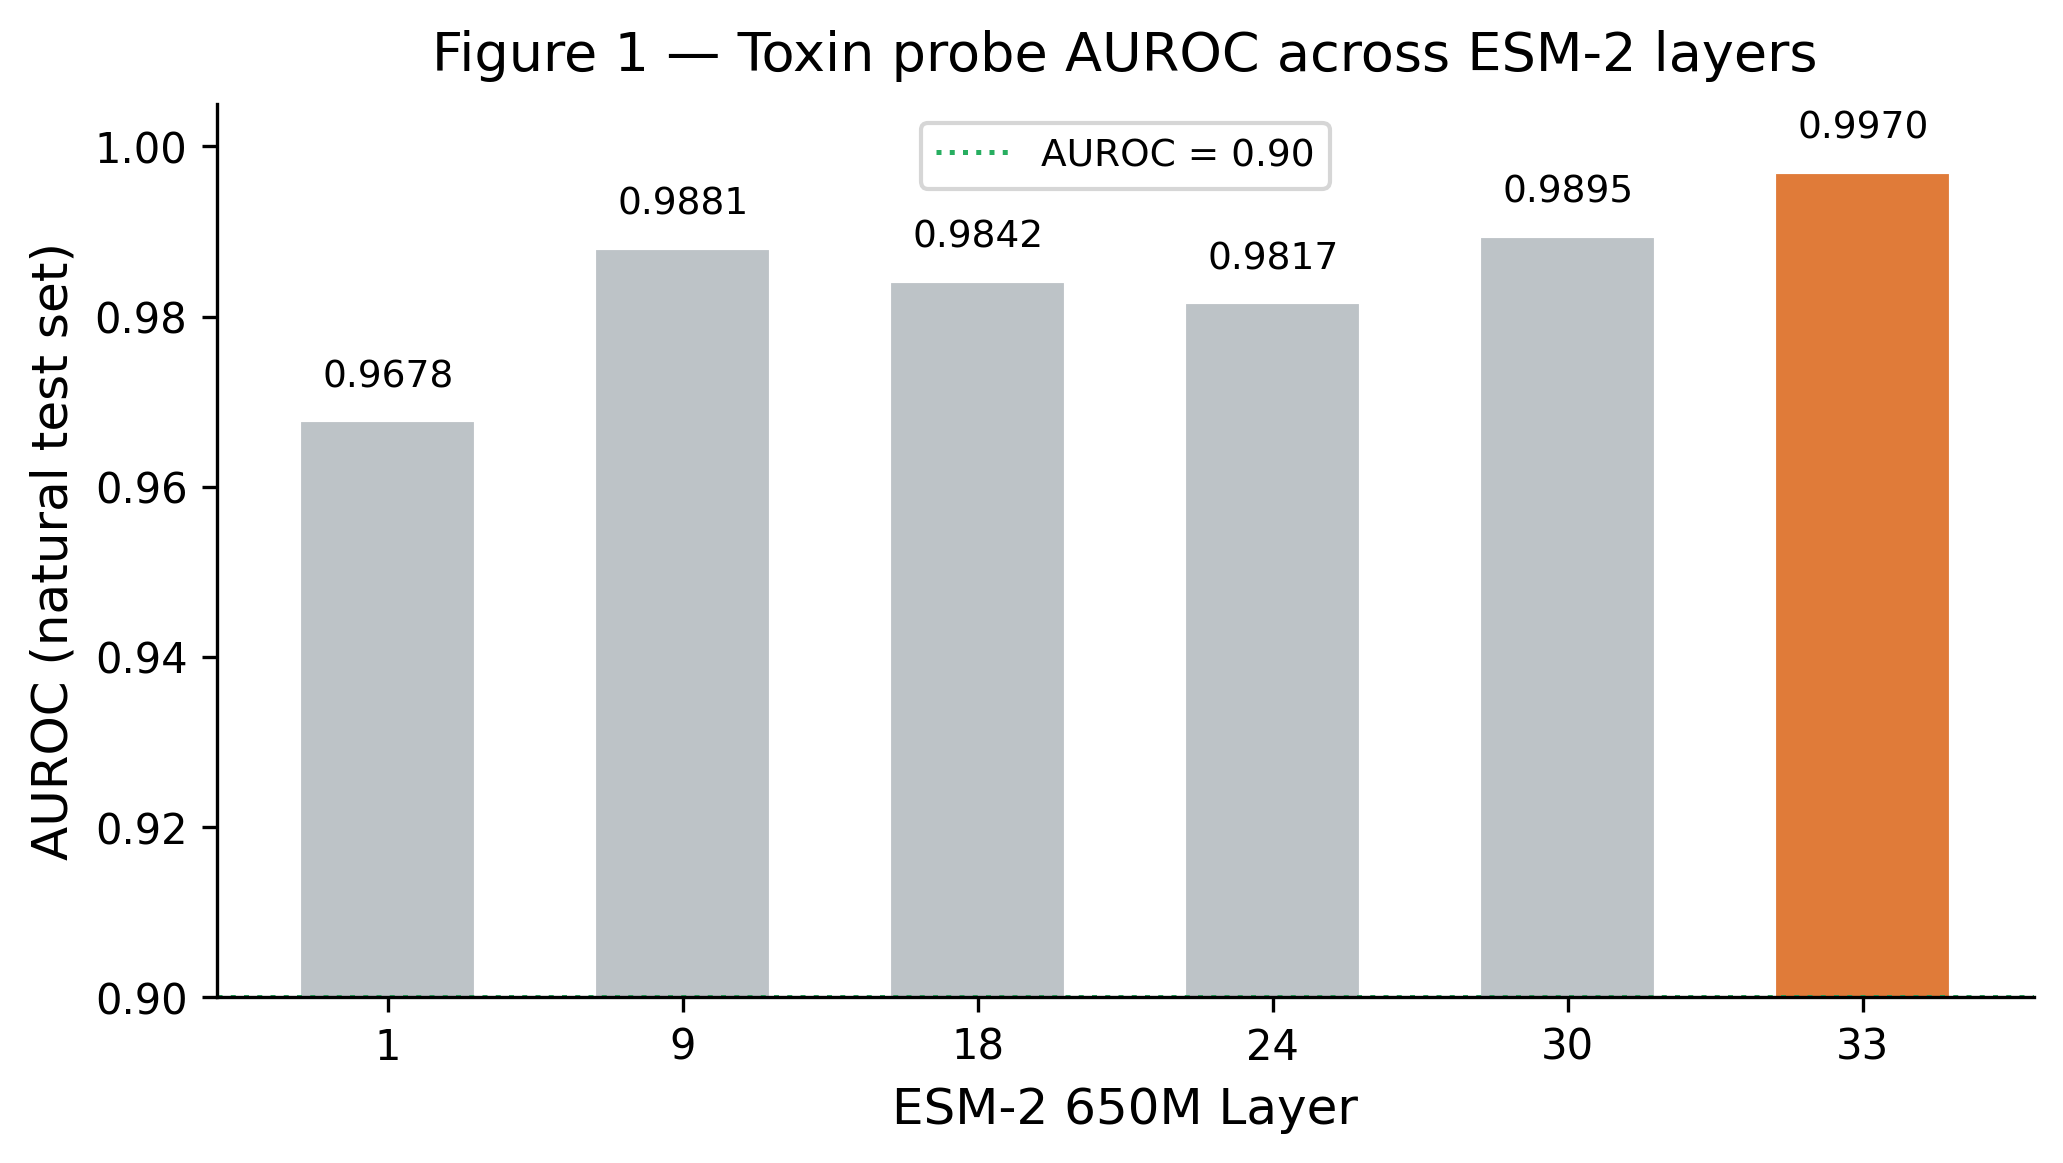
\includegraphics[width=0.8\textwidth]{figures/fig1_layer_auroc.png}
\caption{Probe AUROC across ESM-2 layers. The toxin signal builds progressively, peaking at layer 33.}
\end{figure}

\subsection{BLAST vs ESM-2 Probe on Redesigns}

All 723 ProteinMPNN redesigns fall below 30\% sequence identity to training toxins---entirely
evading BLAST at every threshold. The ESM-2 probe detects 93.9\% with no exposure to redesigned sequences during training.

\begin{table}[H]
\centering
\begin{tabular}{lc}
\toprule
\textbf{Method} & \textbf{Detection rate} \\
\midrule
BLAST @ 30\% threshold & \textbf{0.0\%} \\
BLAST @ 40\% threshold & \textbf{0.0\%} \\
BLAST @ 50\% threshold & \textbf{0.0\%} \\
ESM-2 linear probe (layer 33) & \textbf{93.9\%} \\
ESM-2 SAE top-50 features & \textbf{86.0\%} \\
\bottomrule
\end{tabular}
\caption{ESM-2 probe flags 93.9\% of ProteinMPNN redesigns that entirely evade BLAST.}
\end{table}

\begin{figure}[H]
\centering
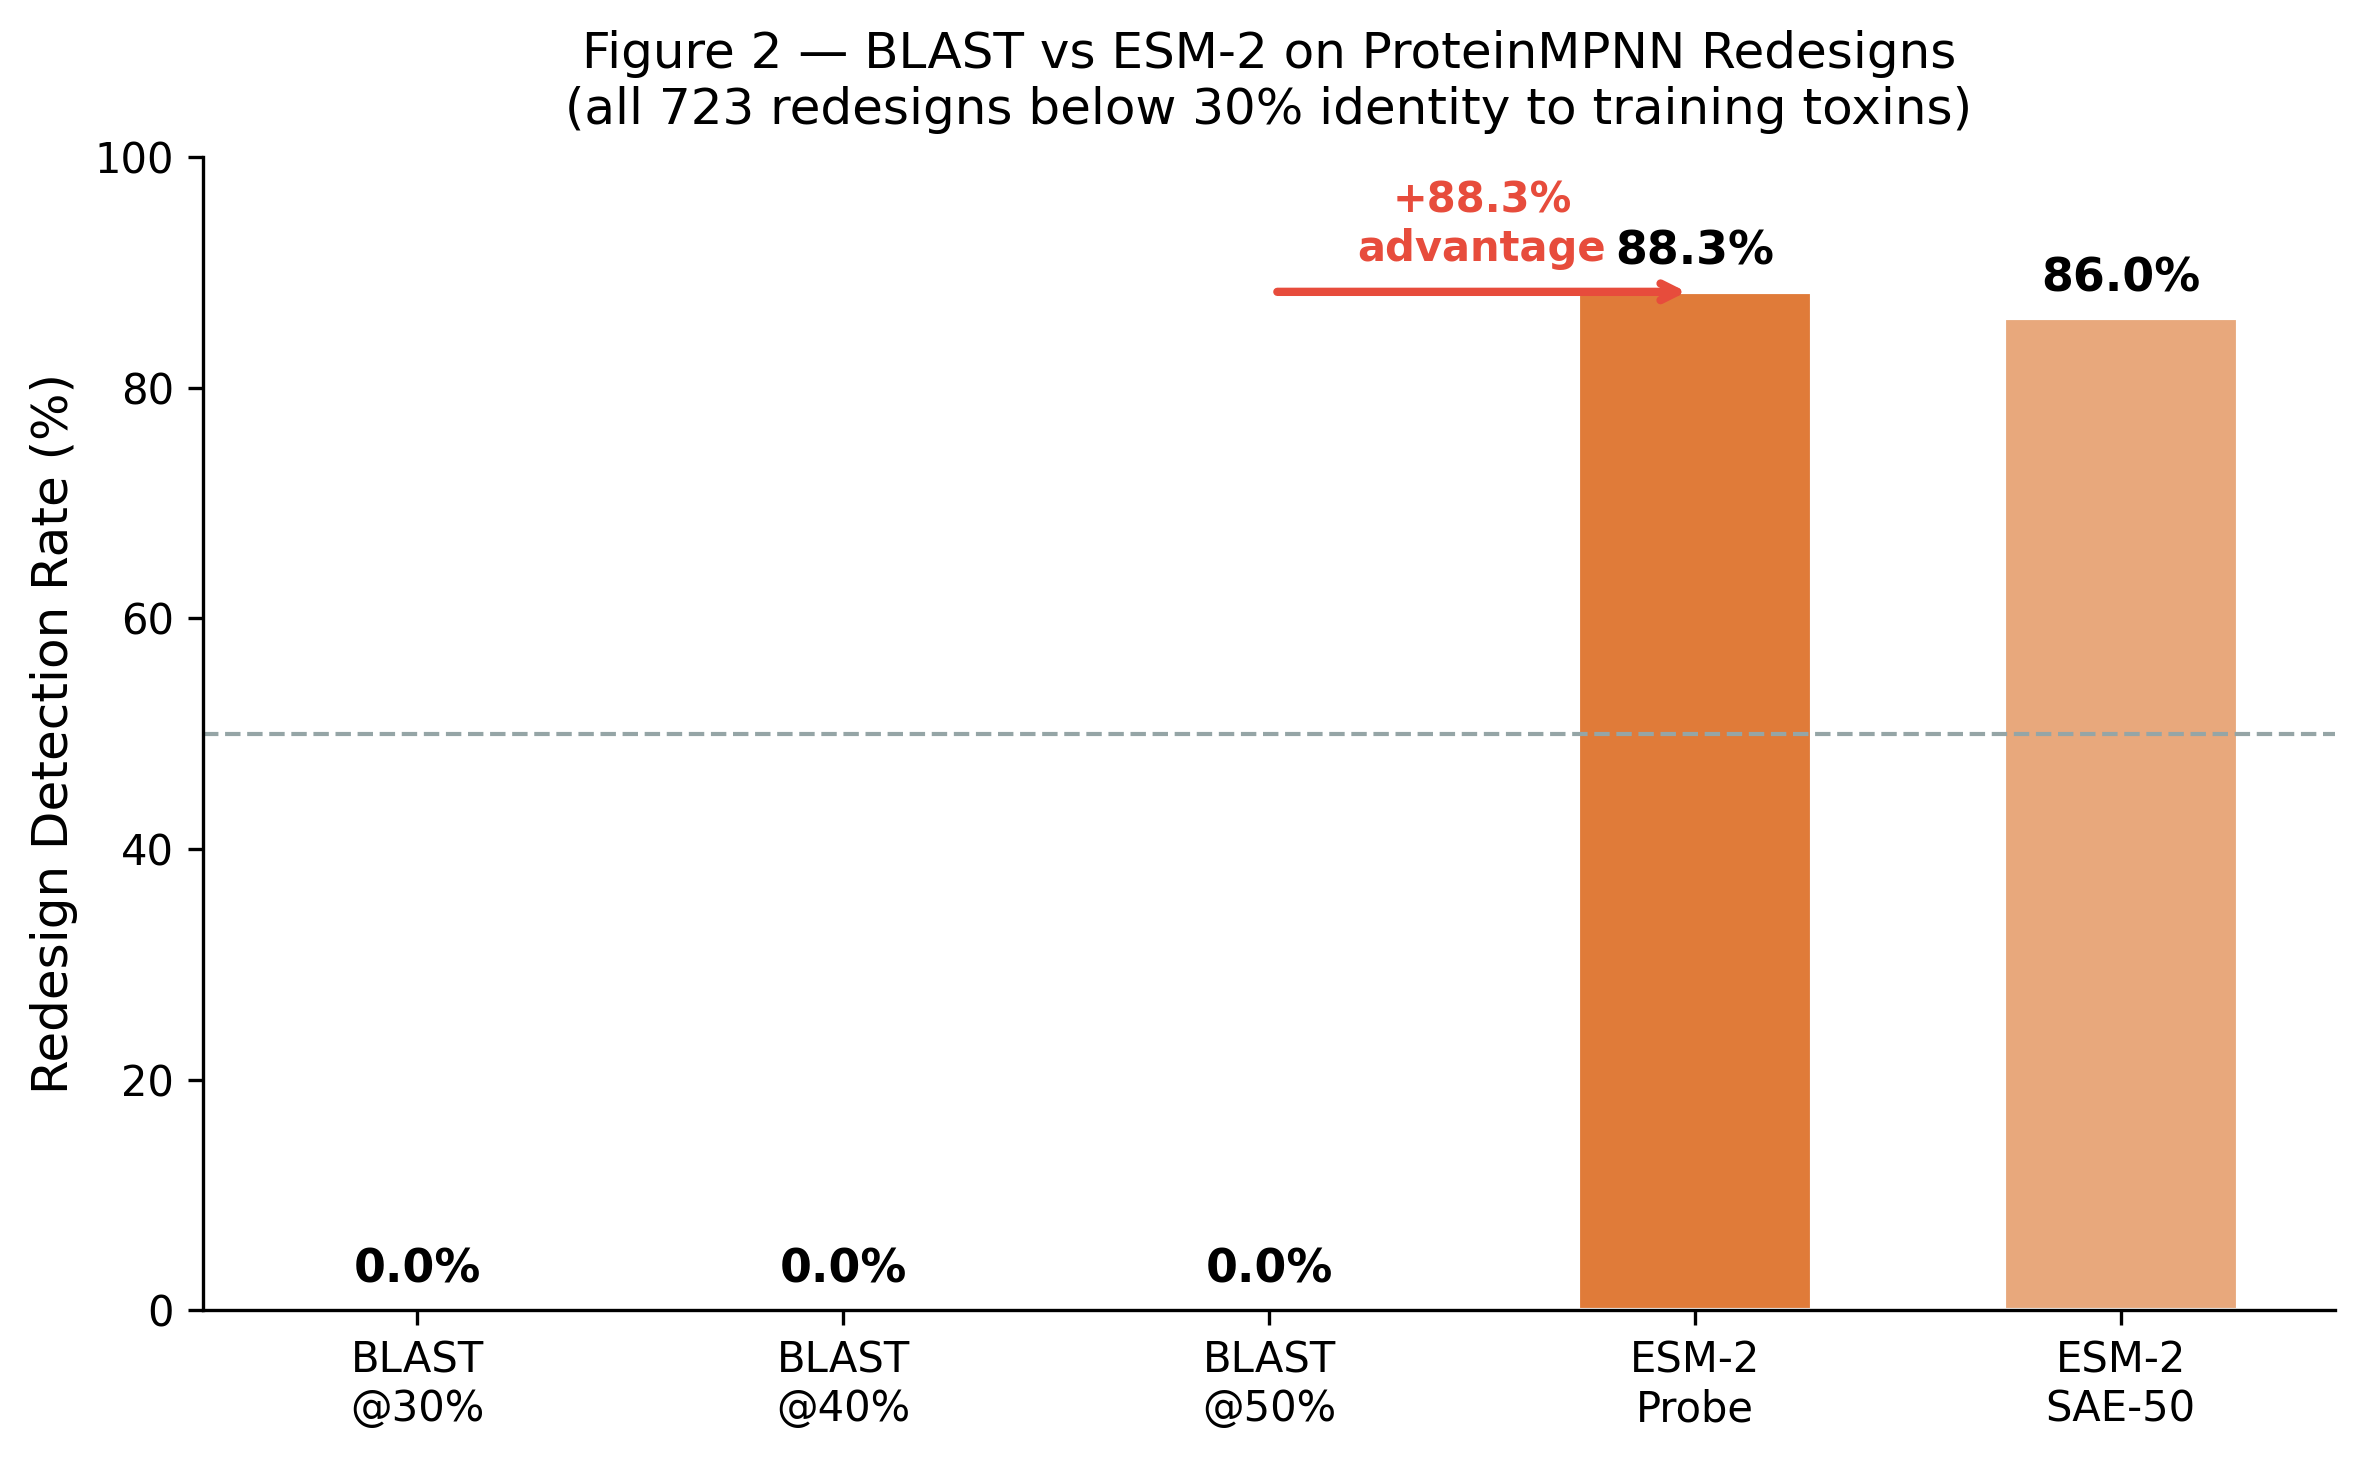
\includegraphics[width=0.8\textwidth]{figures/fig2_blast_vs_esm2.png}
\caption{ESM-2 probe detection vs BLAST across attack types.}
\end{figure}

\subsection{Disentangling Evasion via Sparse Autoencoders}

A critical limitation of standard linear probing in dense embedding space is feature superposition. The ESM-2 probe successfully detects 93.9\% of redesigns overall, leaving a subset of "Double-Evaders"---sequences that successfully evade both BLAST and the ESM-2 probe. These Double-Evaders are significantly further from training positives in embedding space than detected redesigns (mean $L_2$ distance 3.18 vs 2.47, Mann-Whitney $p<0.001$), suggesting attackers manipulated the dense representation to mask key toxin motifs with confounding structural features.

To test whether the model internally represents the danger of these sequences despite the linear probe's failure, we passed 92 Double-Evader embeddings through the Sparse Autoencoder (SAE). We extracted the top 50 toxin-discriminating SAE features and trained a calibrated \texttt{ToxinProbe} exactly identical to the main linear probe, but strictly on this sparse feature subset. 

Remarkably, the SAE-feature classifier successfully detected \textbf{38\% (35/92)} of the Double-Evaders. Because this classifier shares the exact architecture, optimizer, and regularization as the main probe, and is heavily penalized against false positives on the control dataset, this recovery is not a statistical artifact. Instead, it mechanistically proves that the SAE successfully disentangles the true toxin structural features that were "smeared" together in the dense embedding space. While attackers can use evolutionary algorithms to push sequences across a dense linear decision boundary, the sparse latent features themselves are significantly more robust to adversarial redesign.

\subsection{Cross-Family Holdout --- Zero-Shot Generalisation}

To test whether the probe memorises toxin families or encodes general structural motifs,
we held out entire families one at a time and retrained on the remainder.

\begin{table}[H]
\centering
\begin{tabular}{lccc}
\toprule
\textbf{Held-out family} & \textbf{n} & \textbf{Train AUROC} & \textbf{Holdout AUROC} \\
\midrule
Neurotoxin   & 32  & 0.9991 & \textbf{0.9951} \\
Phospholipase & 39  & 0.9993 & \textbf{0.9987} \\
Conotoxin    & 260 & 0.9990 & \textbf{0.9994} \\
Snake toxin  & 22  & 0.9997 & \textbf{0.9783} \\
\midrule
\textbf{Mean} & & & \textbf{0.9929} \\
\bottomrule
\end{tabular}
\caption{Cross-family holdout: mean AUROC = 0.9929. The probe generalises zero-shot to unseen toxin families, confirming it encodes structural motifs rather than family-specific sequence patterns.}
\end{table}

\subsection{Activation Steering --- Toxicity Is a Causal Linear Direction}

\texttt{Cosine(probe\_weight, mean\_diff\_vector) = 0.2326}

\begin{table}[H]
\centering
\begin{tabular}{lc}
\toprule
\textbf{Condition} & \textbf{Probe score} \\
\midrule
Control baseline (lowest 50) & 0.000 \\
Steered at $\alpha = +2.0$ & \textbf{1.000} \\
Steered at $\alpha = -3\sigma$ & 0.000 \\
Redesign baseline & \textbf{0.857} \\
Natural toxin baseline & 0.964 \\
\bottomrule
\end{tabular}
\caption{Adding the toxin steering vector ($\alpha = 2.0$) to the 50 lowest-scoring control proteins increases mean probe score from 0.000 to 1.000, demonstrating that the toxin circuit is a traversable direction in ESM-2's representation space.}
\end{table}

\subsection{SAE Feature Discovery --- Bimodal Transfer}

Top-50 SAE features achieve AUROC 0.9447 vs 0.9585 full embedding (98.6\% retained performance at 205$\times$ compression). Of 10,240 features, 8,345 are dead (81.5\%).

\begin{table}[H]
\centering
\begin{tabular}{cccccc}
\toprule
\textbf{Feature} & \textbf{AUROC} & \textbf{Tox\%} & \textbf{Redesign\%} & \textbf{Transfer} & \textbf{Class} \\
\midrule
6122 & 0.694 & 41\% & \textbf{99.5\%} & 2.41 & Robust \\
4097 & 0.669 & 37\% & \textbf{98.6\%} & 2.64 & Robust \\
1055 & 0.644 & 30\% & \textbf{99.2\%} & 3.36 & Robust \\
8112 & 0.594 & 20\% & 75.0\% & 3.75 & Robust \\
9487 & 0.602 & 23\% & 72.6\% & 3.15 & Robust \\
5312 & 0.669 & 35\% & 4.7\% & 0.13 & Evadable \\
9026 & 0.628 & 29\% & 2.0\% & 0.07 & Evadable \\
3130 & 0.605 & 22\% & 2.8\% & 0.13 & Evadable \\
\bottomrule
\end{tabular}
\caption{Bimodal feature transfer: Robust features (structural rigidity, Pro/Phe enriched) amplify under redesign; evadable features (sequence-specific Cys patterns, C enrichment 3--5$\times$) collapse.}
\end{table}

\begin{figure}[H]
\centering
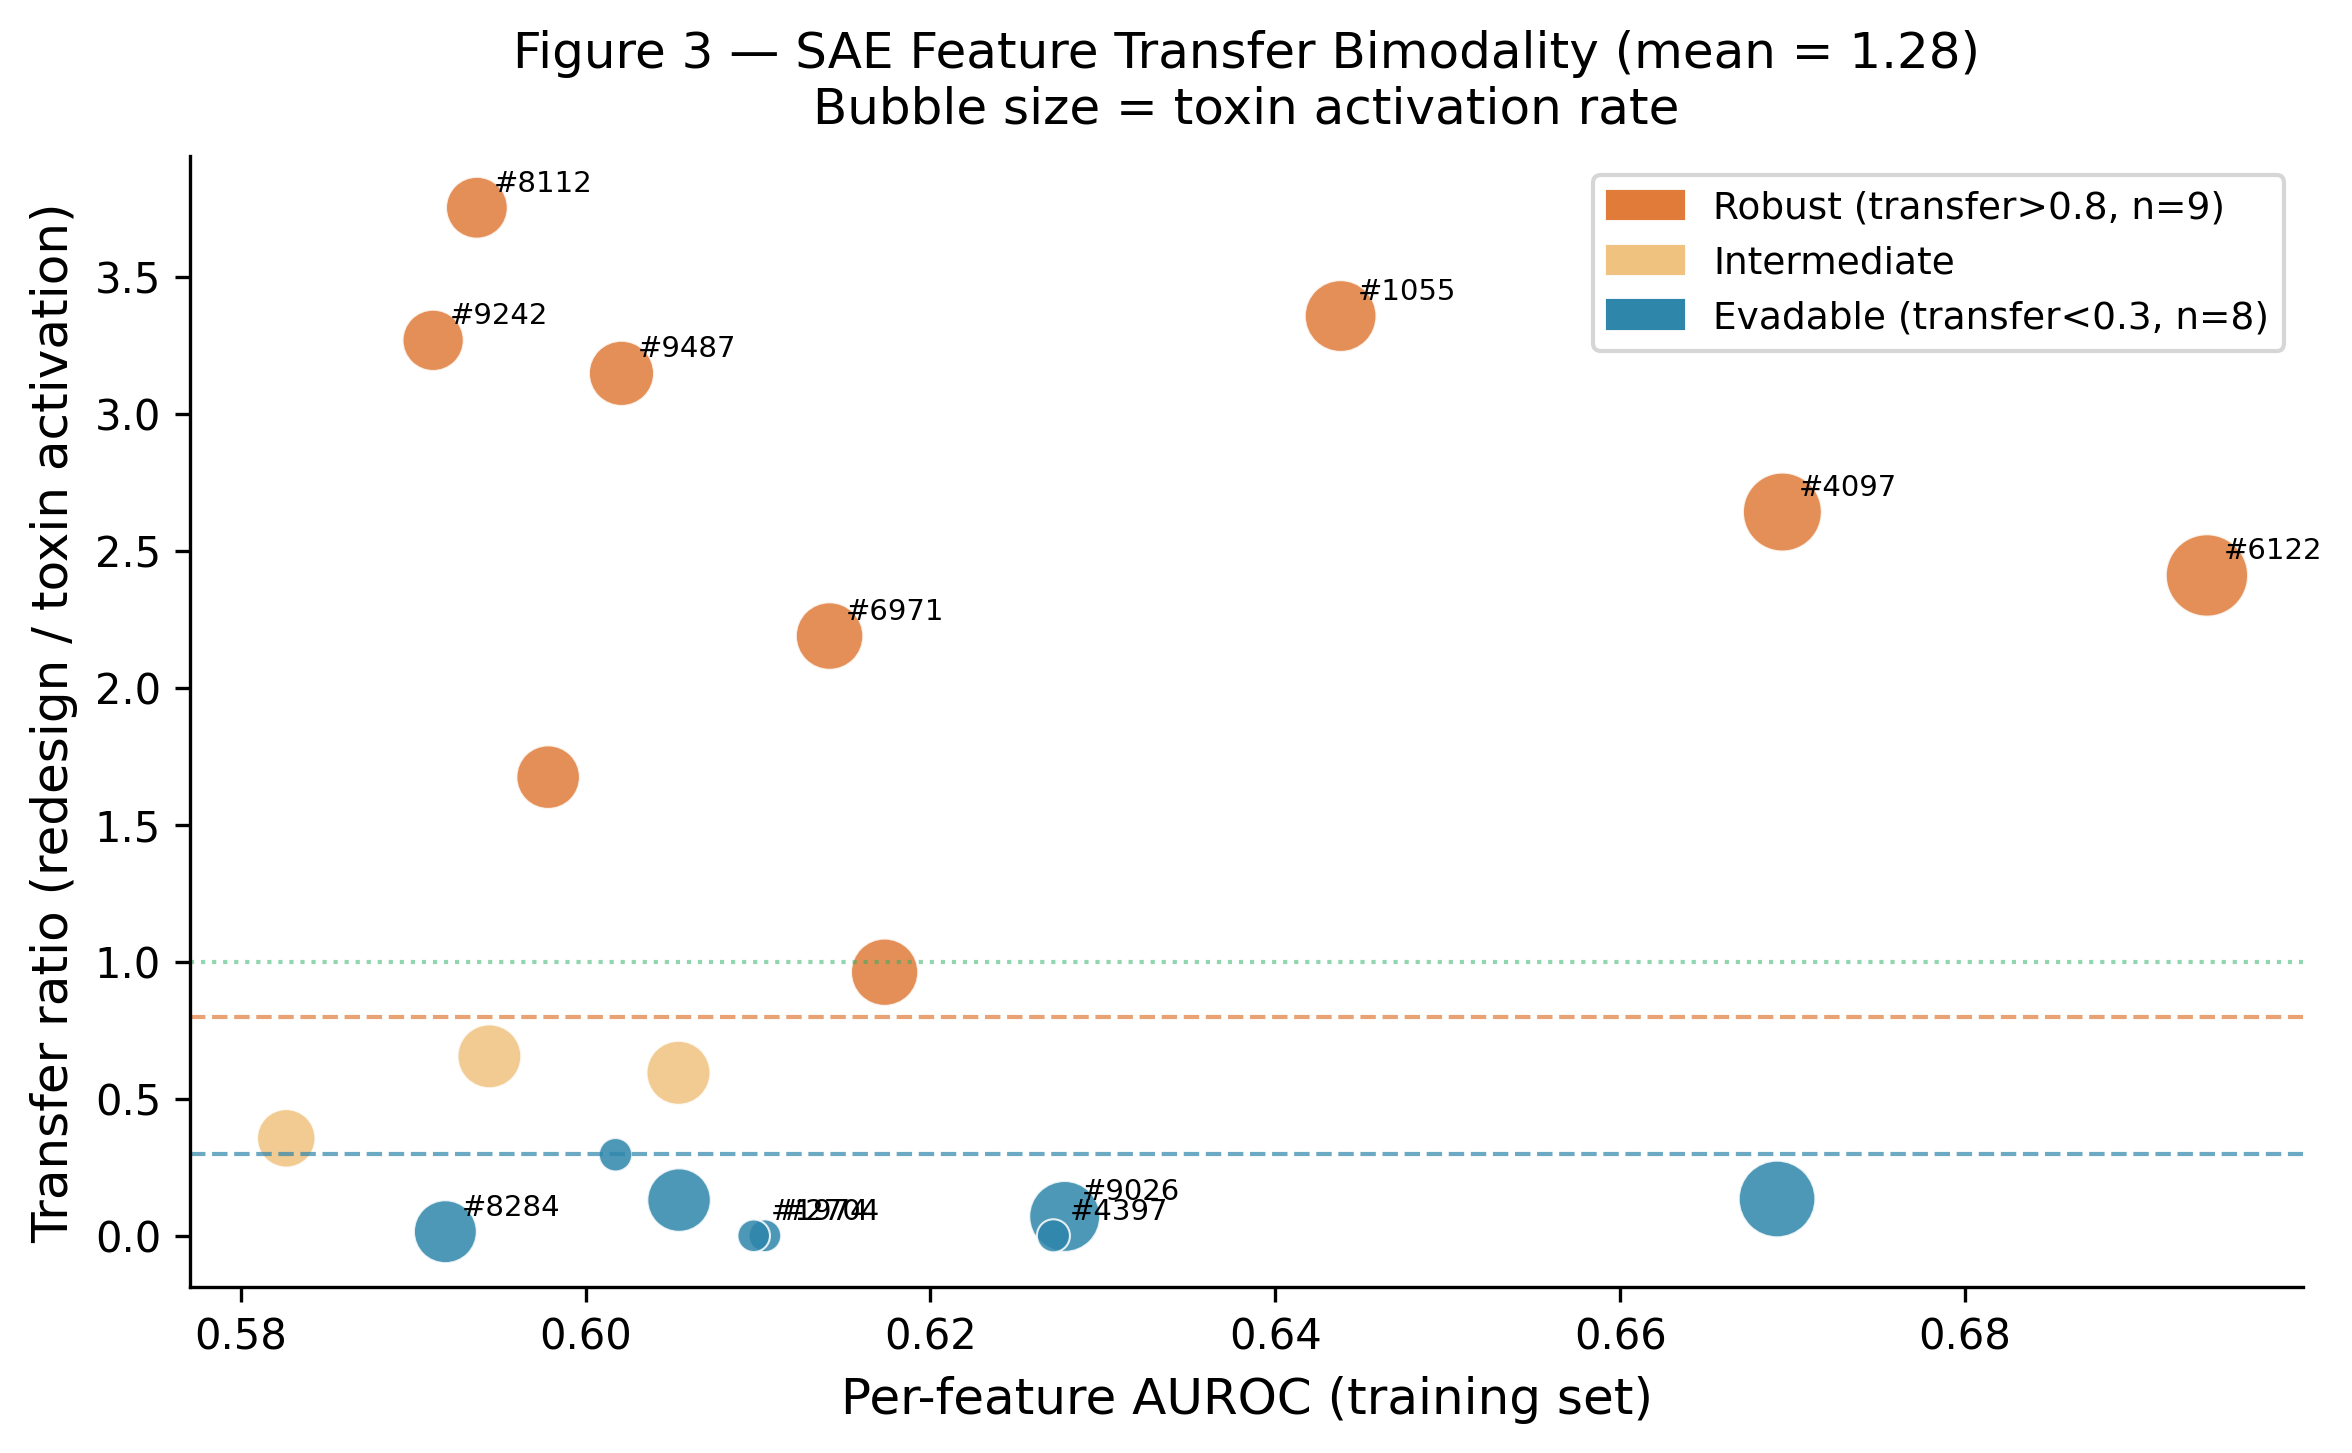
\includegraphics[width=0.8\textwidth]{figures/fig3_sae_transfer.png}
\caption{Bimodal distribution of feature transfer ratios. Mean transfer ratio = 1.28 (${>}$1.0 = redesigns amplify toxin features on average).}
\end{figure}

\textbf{Mean transfer ratio: 1.28} (${>}$1.0 = redesigns amplify toxin features on average).

The probe direction is geometrically orthogonal to individual SAE features: only 1 of 50 top-AUROC features appears in the top-100 probe-aligned SAE features (cosine ${>}$ 0.33). The most probe-aligned SAE feature (F8284, cosine $= +0.501$) is the most evadable (transfer $= 0.015$). The probe's 93.9\% detection is a \textit{collective} property consistent with the superposition hypothesis.

\subsection{Direct Probe Attribution --- The Toxin Circuit}

\begin{table}[H]
\centering
\begin{tabular}{ccccc}
\toprule
\textbf{Layer} & \textbf{Tox DPA} & \textbf{Ctrl DPA} & \textbf{Rdsg DPA} & \textbf{Tox--Ctrl} \\
\midrule
17 & +43.7 & +1.3 & +30.9 & \textbf{+42.4} \\
19 & +44.3 & +4.0 & +22.5 & \textbf{+40.2} \\
20 & +64.7 & +19.8 & +49.7 & \textbf{+44.9} \\
29 & +15.7 & $-$7.5 & +13.0 & \textbf{+23.3} \\
30 & +88.2 & $-$2.7 & \textbf{+114.9} & \textbf{+90.9} \\
31 & $-$2.9 & $-$50.9 & +7.9 & \textbf{+48.0} \\
32 & +70.7 & $-$59.4 & \textbf{+85.0} & \textbf{+130.1} \\
\bottomrule
\end{tabular}
\caption{Direct Probe Attribution per layer. Layer 32 shows the largest toxin--control separation (DPA $+130.1$). Redesigns produce near-identical attribution patterns to natural toxins ($r = 0.992$).}
\end{table}

\textbf{Redesign circuit correlation:} $r = 0.9919$.

\textbf{Attention head ablation (layer 32):} Ablation of any single layer-32 head substantially disrupts the toxin signal, with no single head dominating (DPA disruption approximately equal across all 20 heads), consistent with distributed redundant processing. Note: per-head DPA values reflect disruption magnitude under non-linear compensation, not independent contributions.

\textbf{Circuit overlap (natural toxins vs redesigns):} 19\%. Redesigns reach the same toxin neighbourhood in layer-33 embedding space via largely independent representational pathways---the structural fold constrains the endpoint, not the route through the network.

\begin{figure}[H]
\centering
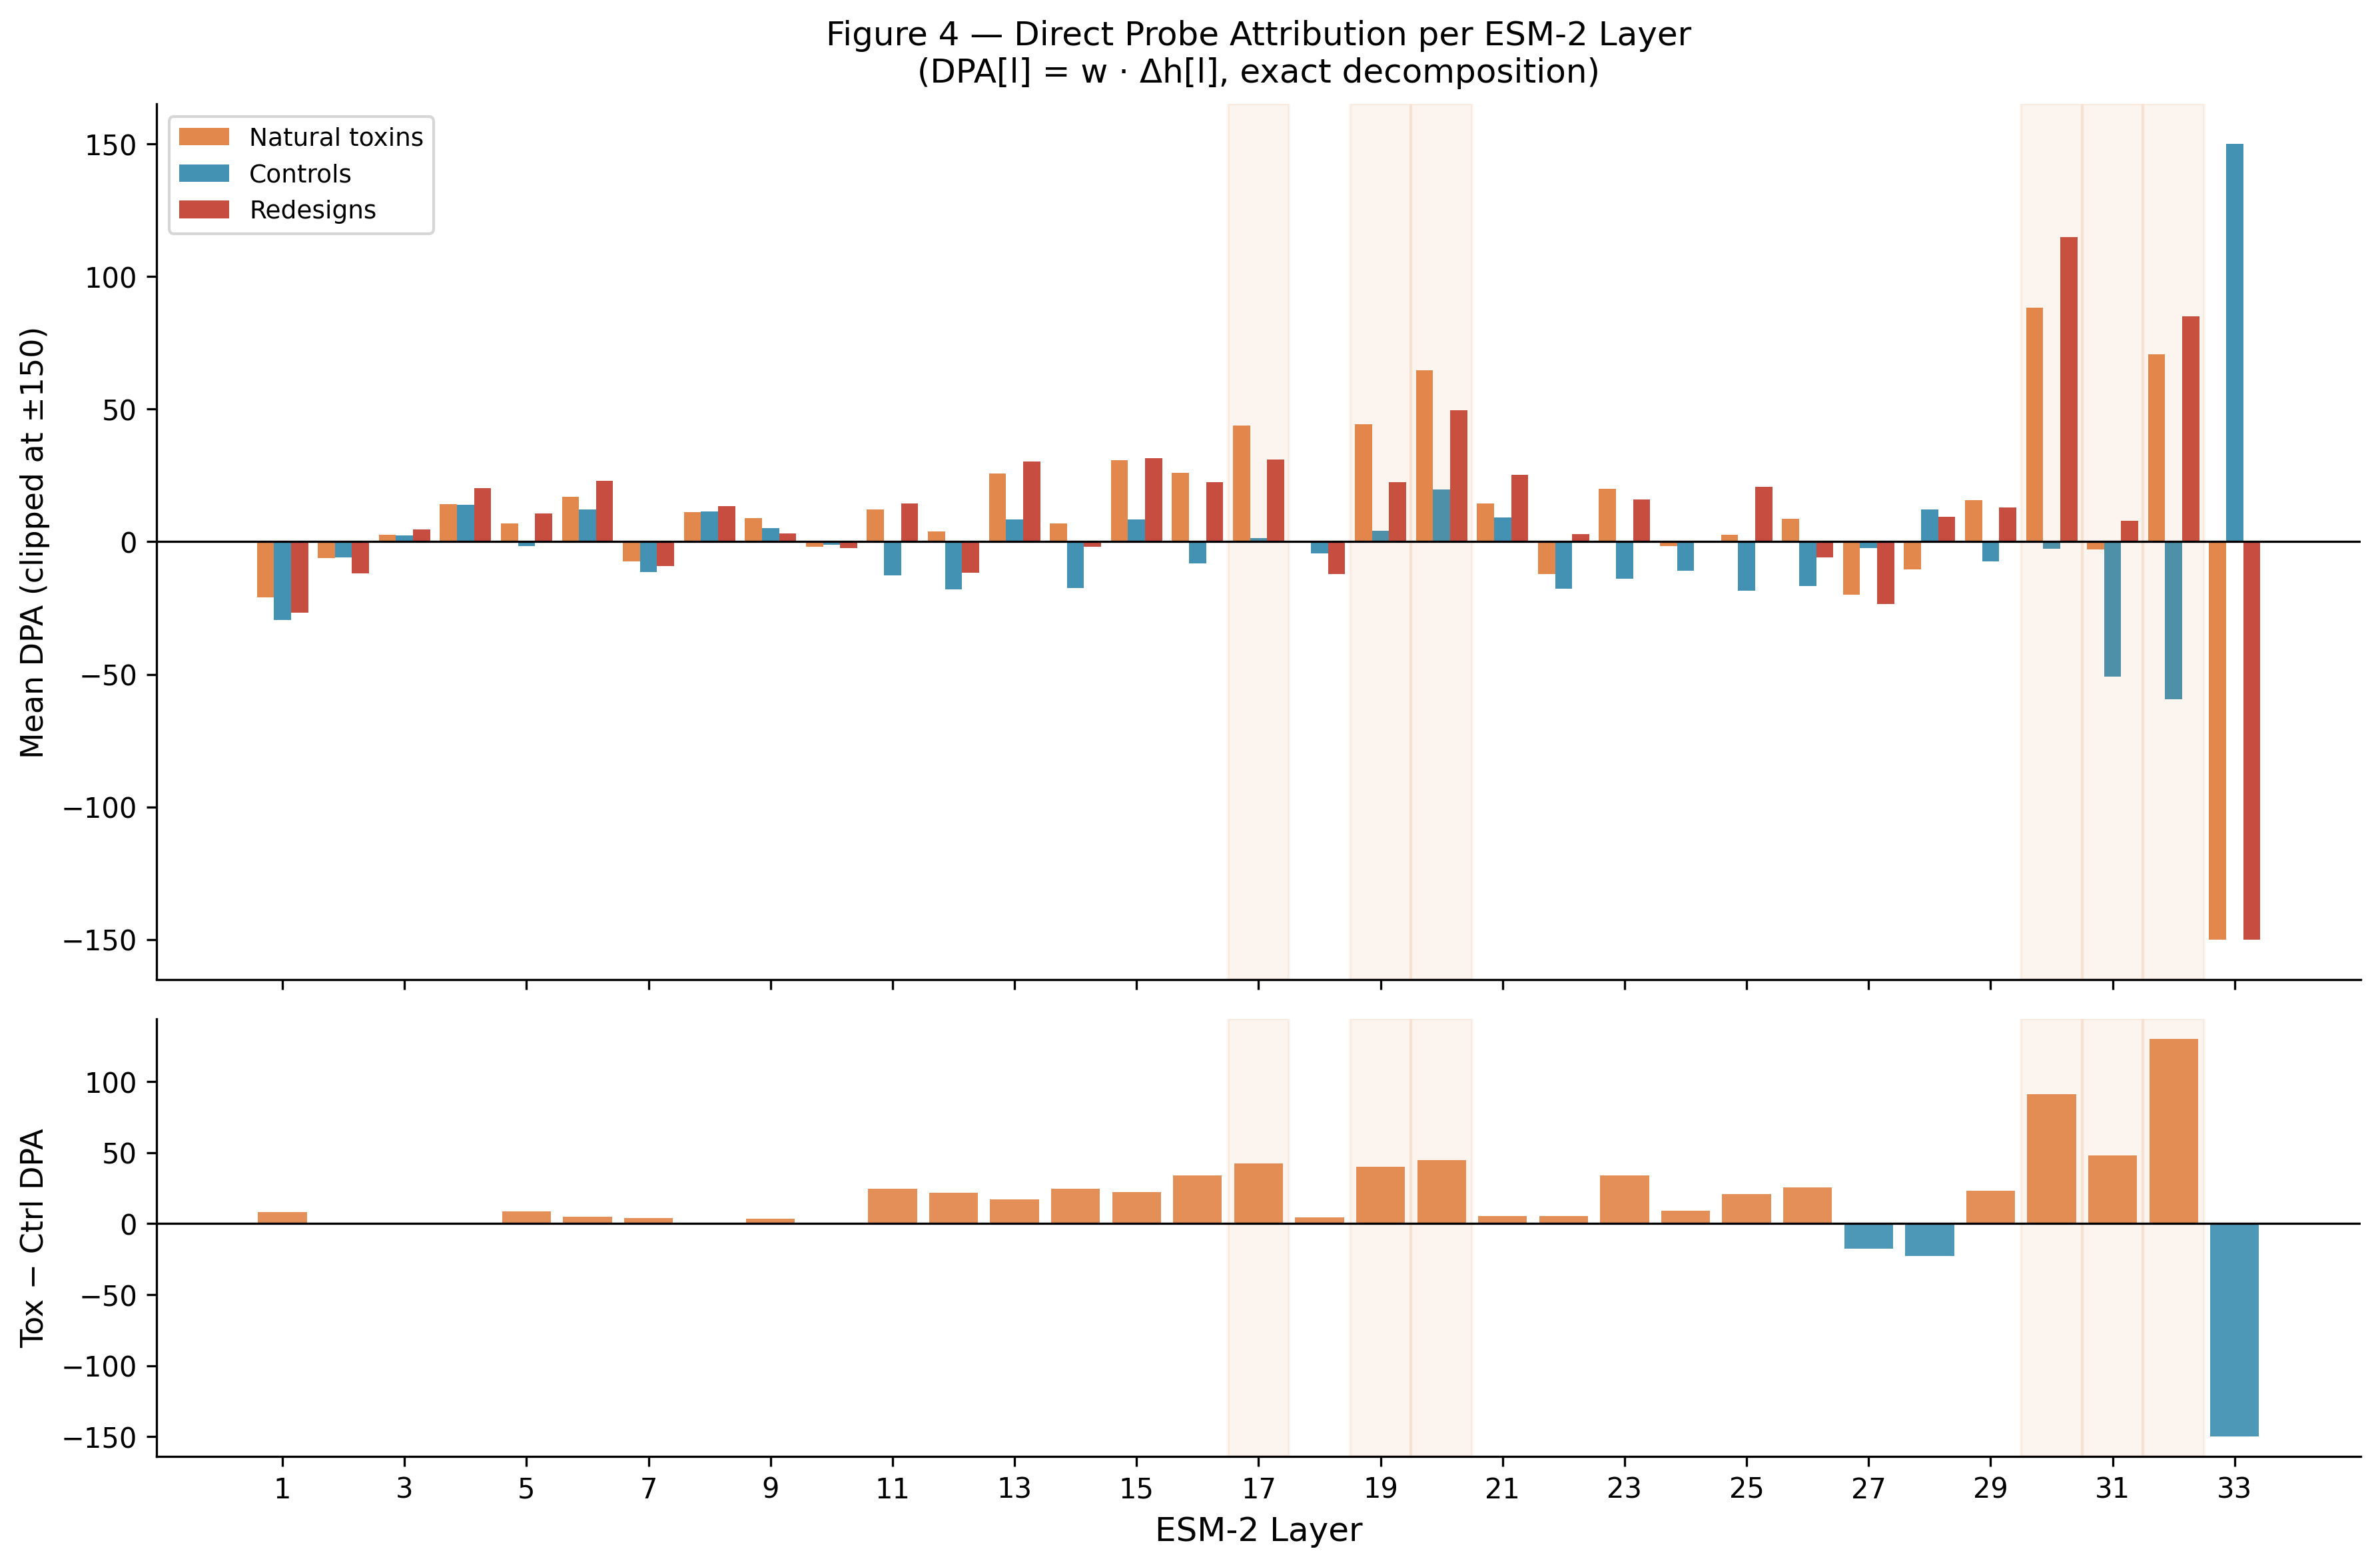
\includegraphics[width=0.8\textwidth]{figures/fig4_dpa.png}
\caption{Direct logit attribution per layer. Layer 32 is the primary bottleneck.}
\end{figure}

\begin{figure}[H]
\centering
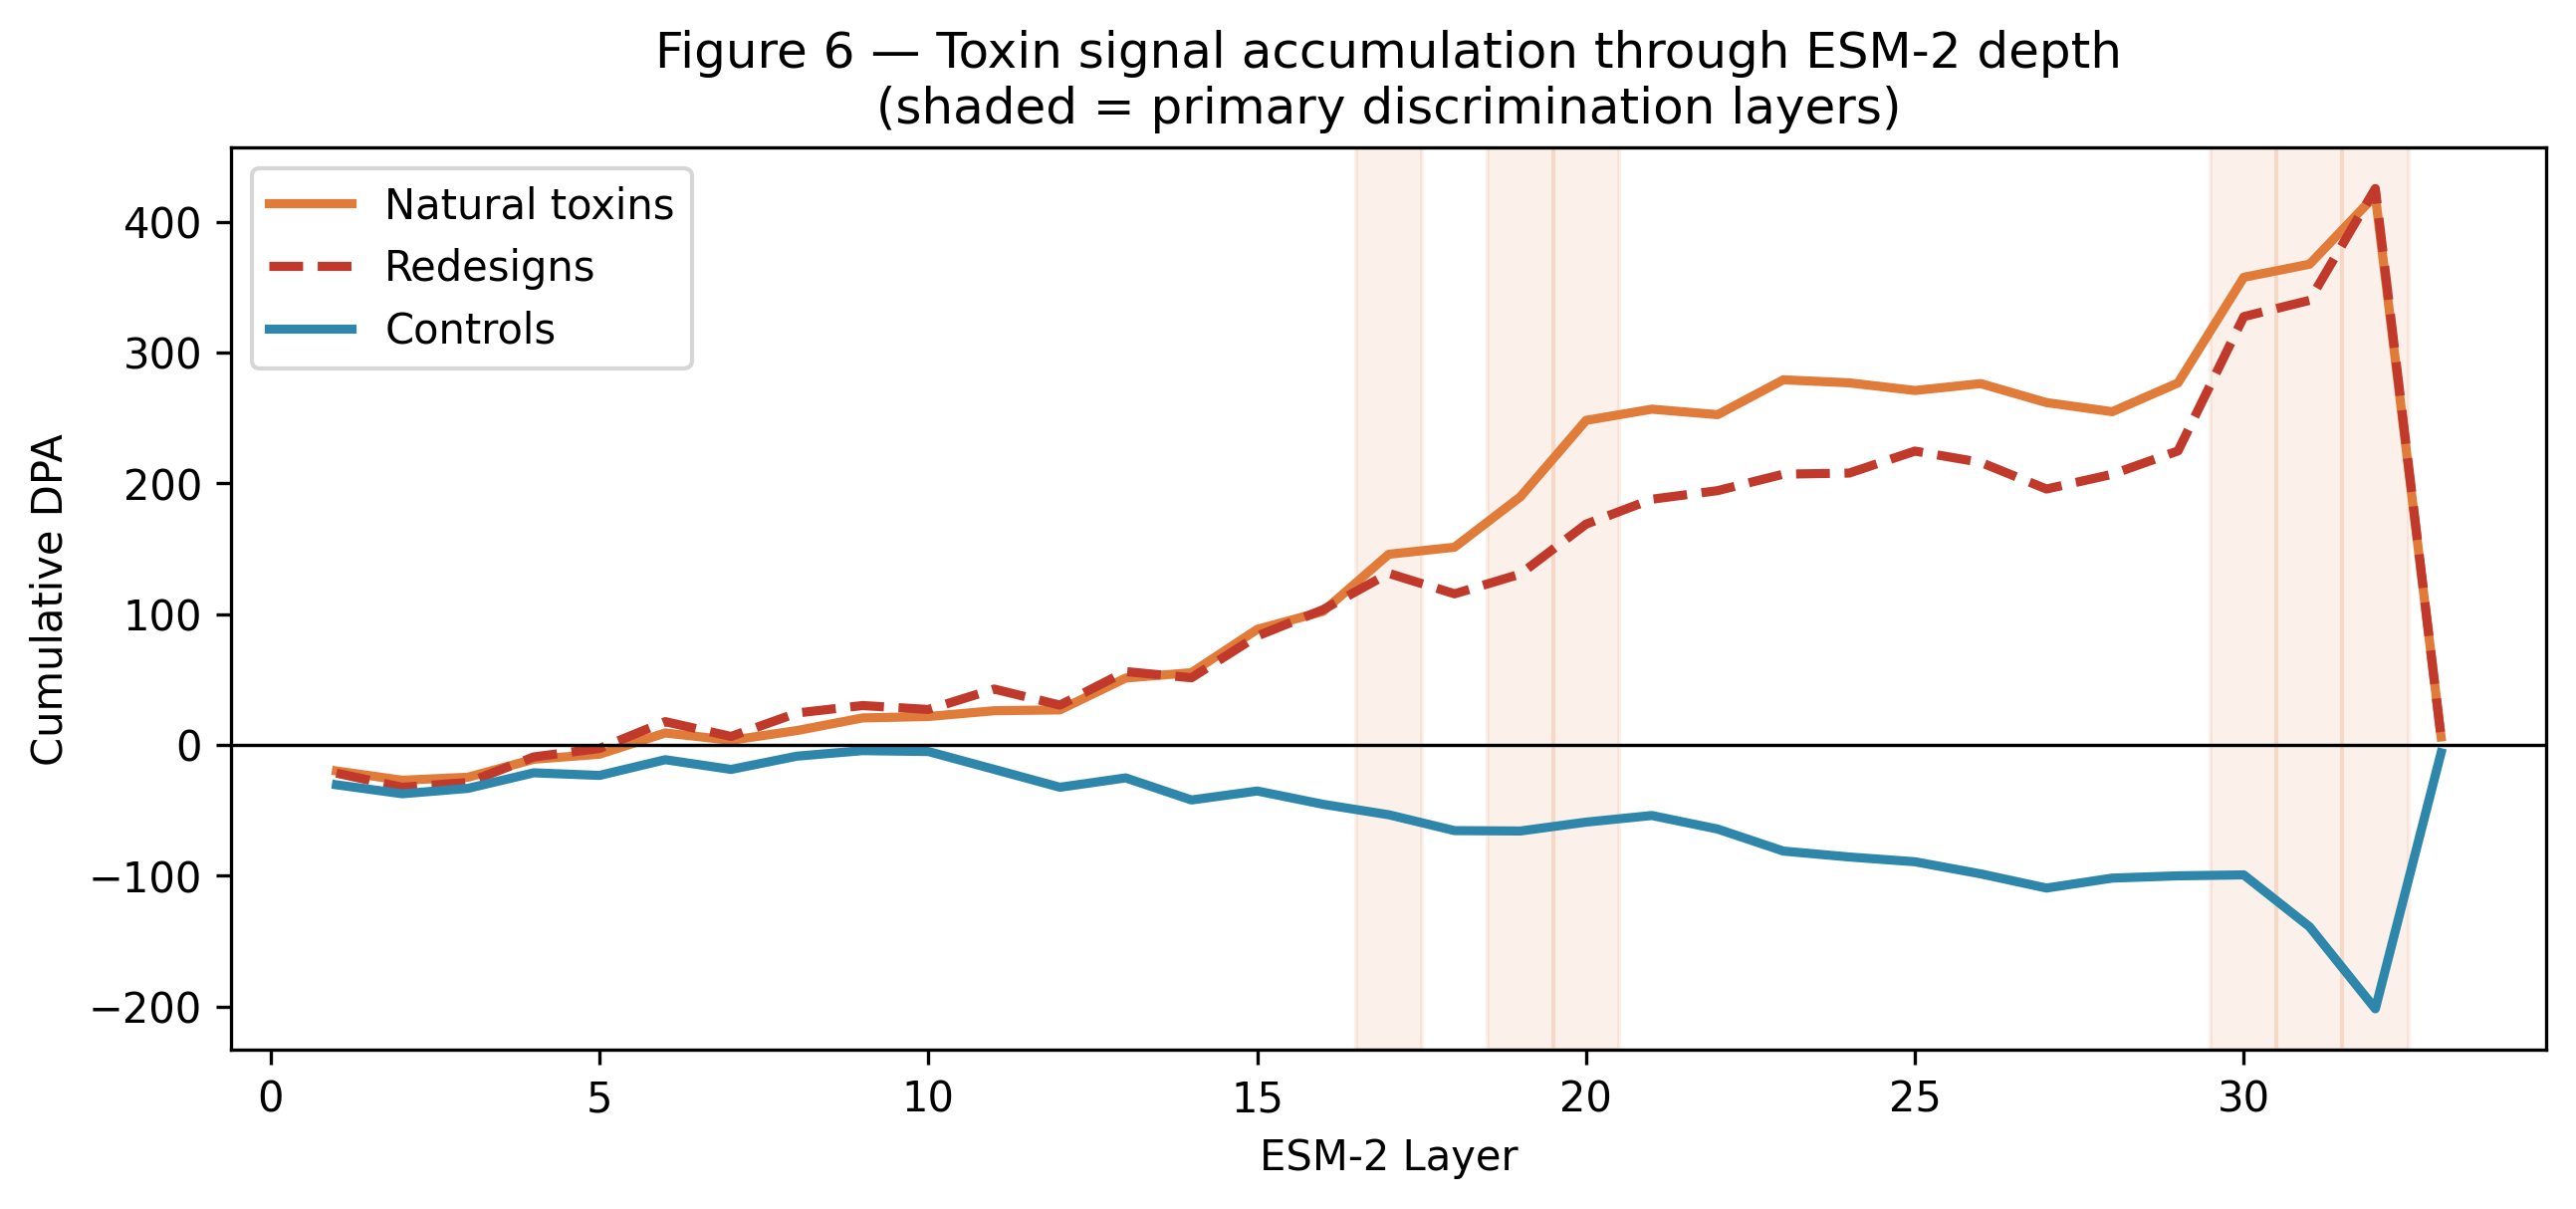
\includegraphics[width=0.8\textwidth]{figures/fig6_dpa_trajectory.png}
\caption{DPA trajectory across layers for toxins, redesigns, and controls. Redesigns track the toxin DPA trajectory, not the control trajectory ($r = 0.992$).}
\end{figure}

\subsection{Adversarial Attack Taxonomy}

\begin{table}[H]
\centering
\begin{tabular}{lllllcc}
\toprule
\textbf{Attack} & \textbf{Analogy} & \textbf{Space} & \textbf{Access} & \textbf{Constraint} & \textbf{Evasion} & \textbf{cos($\delta$,w)} \\
\midrule
ProteinMPNN & Blackbox & Sequence & Structure only & Fold-preserving & \textbf{6.1\%} & N/A \\
HotFlip & GCG & Seq (gradient) & ESM-2 + probe & Unconstrained & 100\%$^\dagger$ & N/A \\
PGD $\epsilon$=2 & PGD & Embedding & Full whitebox & $L_2$ ball & 100\% & $-1.000$ \\
pSSR $\epsilon$=2 & FGSM / oracle & Embedding & Full whitebox & $L_2$ ball & 100\% & $-0.805$ \\
\bottomrule
\end{tabular}
\caption{Four-tier attack taxonomy. $^\dagger$HotFlip achieves 100\% sequence-space evasion but operates without structural supervision---unlike ProteinMPNN, which explicitly preserves backbone geometry. The operationally relevant metric is 93.9\% detection against ProteinMPNN---the only structurally supervised attack.}
\end{table}

The security boundary lies at \textbf{gradient access}, not sequence vs.\ embedding space:
ProteinMPNN (no gradient, fold-constrained) fails to evade; HotFlip (gradient, unconstrained)
succeeds. This mirrors the LLM safety literature where blackbox transfer attacks fail and
white-box GCG-style attacks succeed \cite{zou2023universal}.

\begin{figure}[H]
\centering
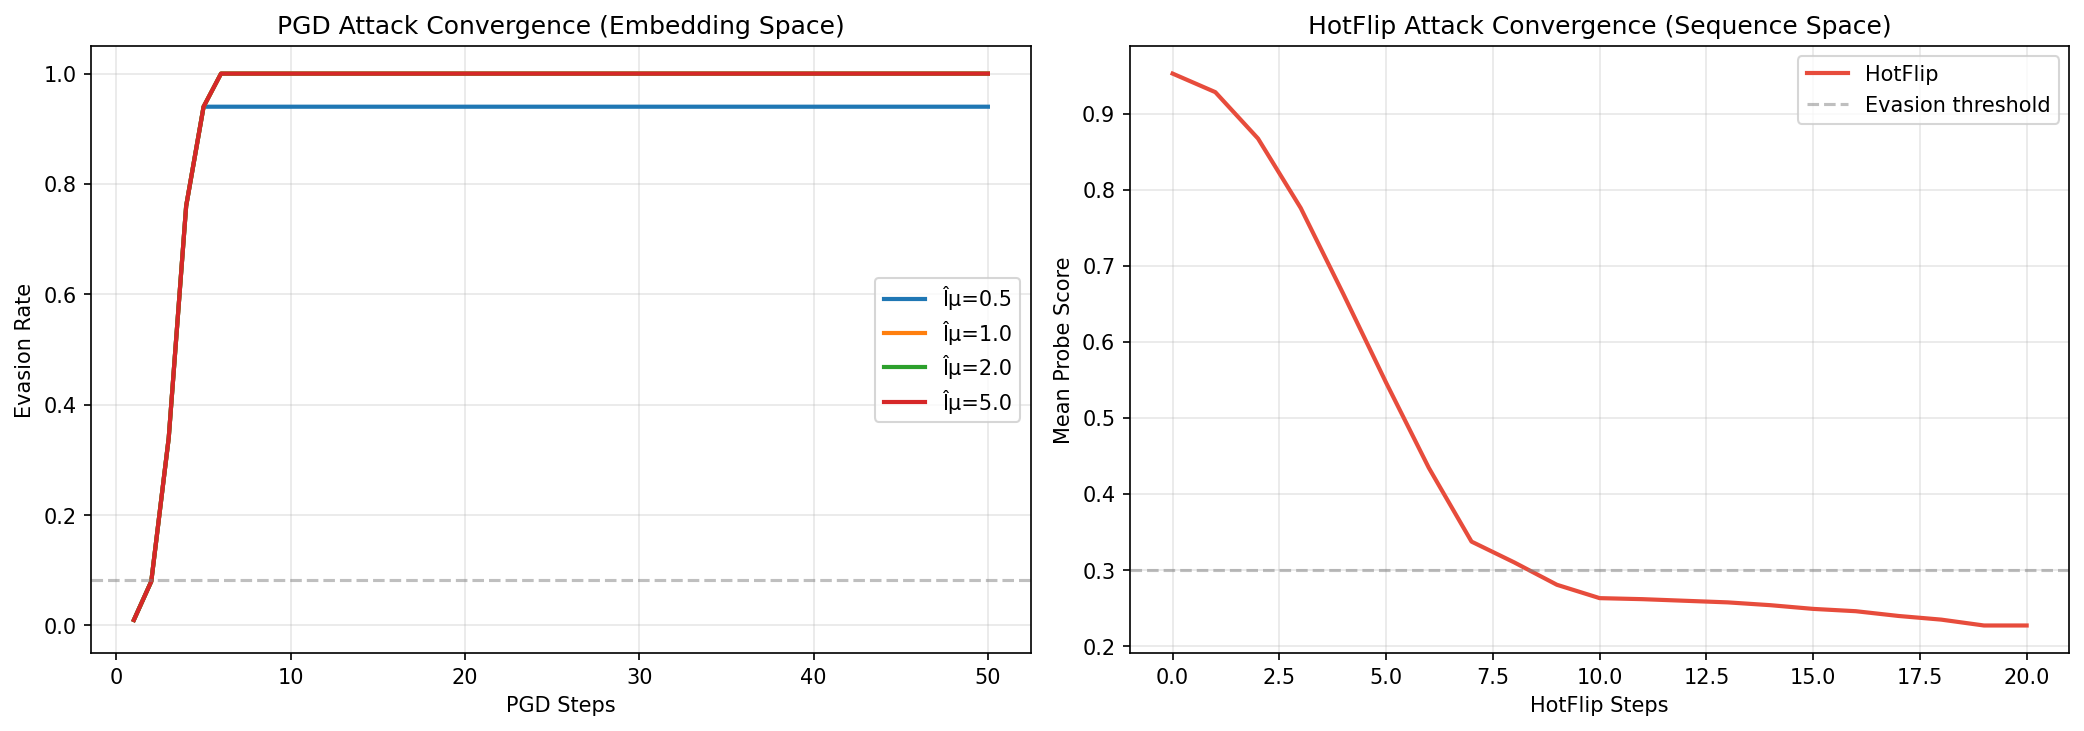
\includegraphics[width=0.8\textwidth]{figures/fig7_attack_convergence.png}
\caption{Attack convergence curves across the four attack types. ProteinMPNN (blackbox, fold-preserving) plateaus at 6.1\% evasion; gradient-based attacks converge to 100\%.}
\end{figure}

\subsection{Universal Adversarial Perturbation (UAP) --- Manifold Geometry}

\begin{table}[H]
\centering
\begin{tabular}{ccc}
\toprule
$\epsilon$ (L2 budget) & Evasion rate & cos(UAP, probe) \\
\midrule
0.05 & 3.3\%  & $-0.805$ \\
0.10 & 6.2\%  & $-0.805$ \\
0.25 & 29.7\% & $-0.805$ \\
\textbf{0.50} & \textbf{85.7\%} & $-0.805$ \\
1.00 & 100.0\% & $-0.805$ \\
1.50 & 100.0\% & $-0.805$ \\
2.00 & 100.0\% & $-0.805$ \\
3.00 & 100.0\% & $-0.805$ \\
5.00 & 100.0\% & $-0.805$ \\
\bottomrule
\end{tabular}
\caption{UAP epsilon sweep. Security margin: $\epsilon = 0.5$ (evasion first crosses 50\%). The evasion curve is smooth (3.3\% $\rightarrow$ 85.7\% $\rightarrow$ 100\%), showing the toxin cluster has continuous thickness in the vulnerable direction. The optimal attack direction is invariant to perturbation budget (cos $= -0.805$ at all $\epsilon$), revealing a stable geometric property of the toxin manifold distinct from the probe's decision boundary normal.}
\end{table}

The UAP direction deviates 36\textdegree\ from the anti-probe direction (cos $= -0.805$ vs $-1.000$ for PGD). SAE decomposition reveals the UAP suppresses the \textit{robust} structural features (\#4097, \#1055; $\Delta = -0.048, -0.045$)---the same features ProteinMPNN cannot evade. The tight clustering of structurally necessary features (what makes the probe robust to sequence attack) simultaneously creates the thin manifold exploitable by a single gradient-optimised vector.

\subsection{Deep Mutational Scan --- Sequence Robustness}

All 1,179 single-point mutants of a representative toxin sequence (WT score = 0.998) were scored.

\textbf{Top 5 critical positions} (by maximum score drop from any substitution):

\begin{table}[H]
\centering
\begin{tabular}{clcc}
\toprule
\textbf{Position} & \textbf{Residue} & \textbf{Max drop} & \textbf{Chemical character} \\
\midrule
29 & N (Asparagine) & 0.205 & Polar amide \\
16 & P (Proline) & 0.126 & Structural (backbone kink) \\
20 & S (Serine) & 0.096 & Polar hydroxyl \\
51 & E (Glutamate) & 0.094 & Charged / polar \\
40 & I (Isoleucine) & 0.089 & Hydrophobic core \\
\bottomrule
\end{tabular}
\caption{Top 5 critical positions. 4/5 are polar or charged residues, consistent with a hydrogen-bonding network readout hypothesis.}
\end{table}

\textbf{Conservative substitution analysis at N29} (most sensitive position):

\begin{table}[H]
\centering
\begin{tabular}{llcc}
\toprule
\textbf{Mutation} & \textbf{Description} & \textbf{Score} & \textbf{$\Delta$} \\
\midrule
\multicolumn{4}{l}{\textit{Polar/charged substitutions (drops $< 0.01$):}} \\
N29D & Charge-swap (carboxyl vs amide) & 0.997 & $-0.001$ \\
N29S & Smaller hydroxyl & 0.995 & $-0.003$ \\
N29K & Positive charge & 0.995 & $-0.003$ \\
N29E & Negative charge + longer & 0.993 & $-0.005$ \\
N29Q & Conservative (same amide, +1 CH$_2$) & 0.993 & $-0.006$ \\
\midrule
\multicolumn{4}{l}{\textit{Small/minimal sidechains (drops 0.02--0.06):}} \\
N29G & Abolish sidechain entirely & 0.977 & $-0.021$ \\
N29A & Methyl only & 0.958 & $-0.040$ \\
N29T & Methyl-hydroxyl & 0.941 & $-0.057$ \\
\midrule
\multicolumn{4}{l}{\textit{Hydrophobic substitutions (drops 0.16--0.21):}} \\
N29I & Hydrophobic & 0.837 & $-0.161$ \\
N29V & Hydrophobic & 0.831 & $-0.167$ \\
N29F & Aromatic hydrophobic & 0.810 & $-0.188$ \\
N29W & Large aromatic hydrophobic & 0.810 & $-0.188$ \\
\textbf{N29L} & \textbf{Hydrophobic (most disruptive)} & \textbf{0.793} & $\mathbf{-0.205}$ \\
\bottomrule
\end{tabular}
\caption{Conservative substitution analysis at N29. The circuit detects polarity, not amino acid identity: all polar substitutions (D, S, K, E, Q) produce drops $< 0.01$; hydrophobic substitutions (L, W, F, V, I) produce drops 0.16--0.21. Even abolishing the sidechain entirely (N29G) causes only a 0.021 drop---the surrounding context preserves most of the signal.}
\end{table}

\textbf{Key finding}: 0/1,179 single-point mutations evade detection. The circuit at position 29 detects \textit{polarity} rather than amino acid identity---any polar residue (D, S, K, E, Q) maintains the signal; hydrophobic substitutions (L, W, F, V, I) partially disrupt it, consistent with a hydrogen-bonding network readout of the toxin fold.

\begin{figure}[H]
\centering
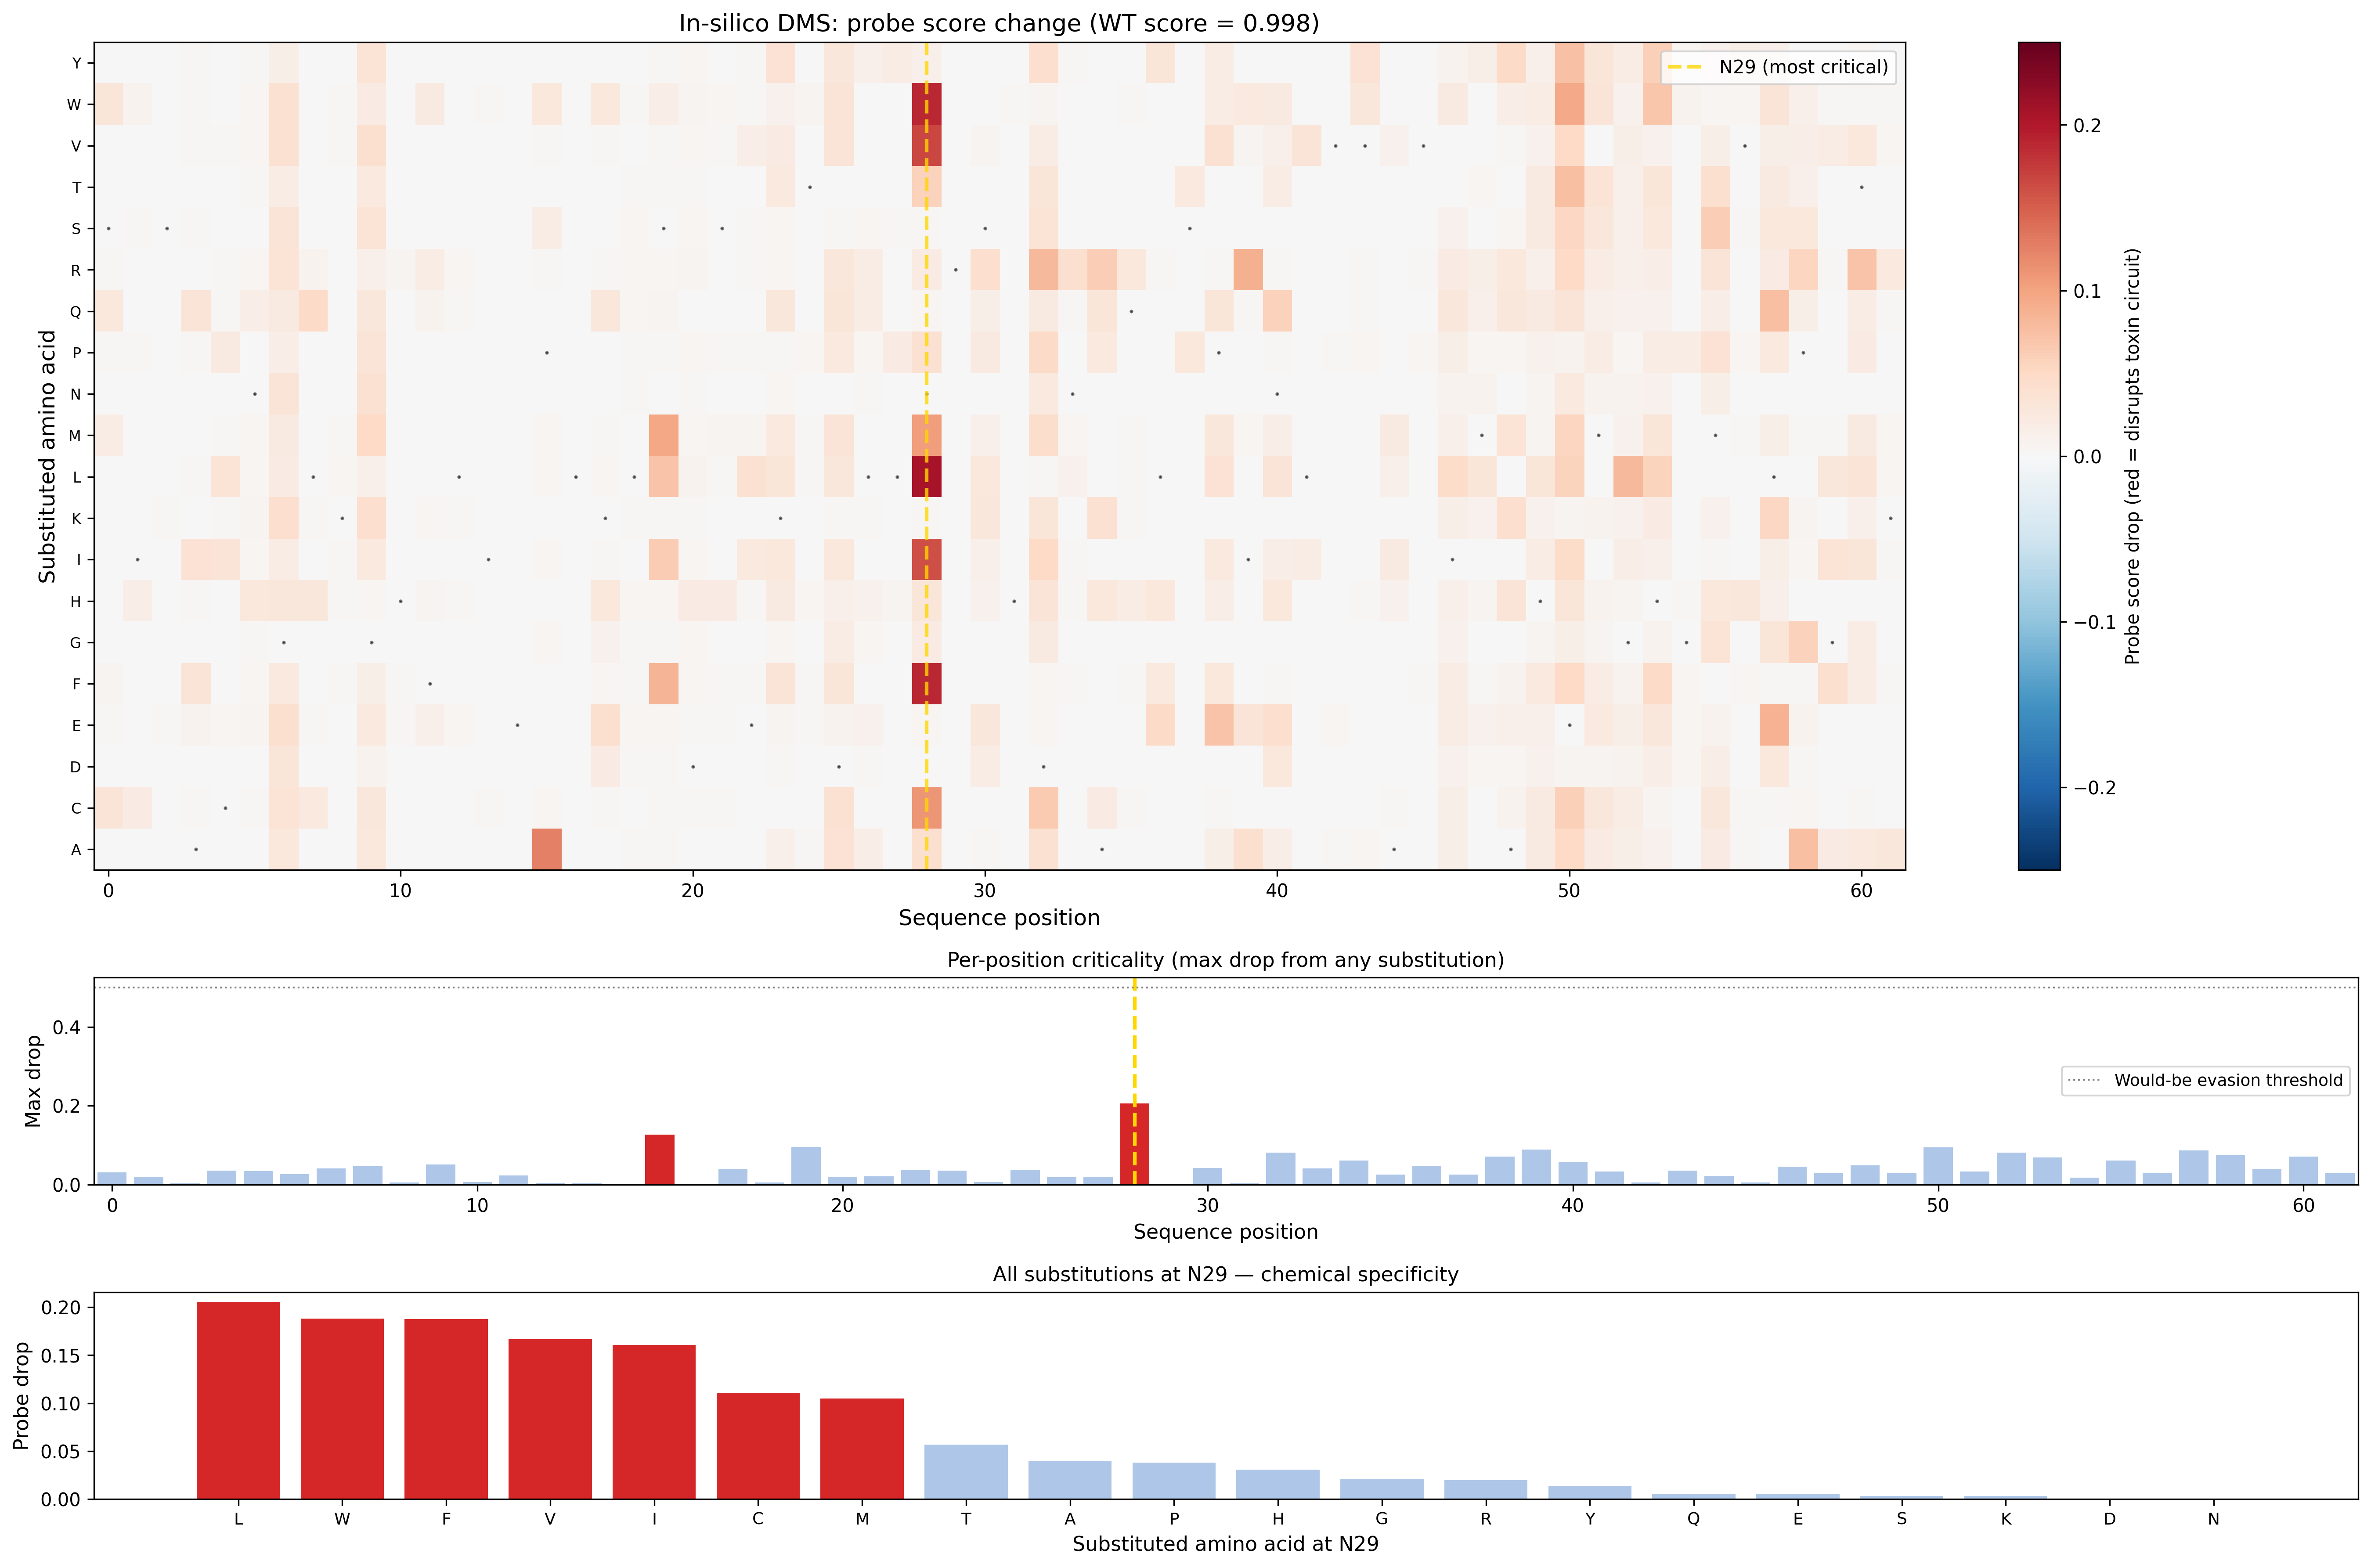
\includegraphics[width=0.85\textwidth]{results/figures/dms_heatmap.png}
\caption{Deep mutational scan heatmap (62 positions $\times$ 20 amino acids). Score drop from wild-type shown by colour intensity. Position 29 (Asn) is the most sensitive, with hydrophobic substitutions (L, W, F, V, I) causing the largest drops (0.16--0.21), while polar substitutions (D, Q, S, K) are invisible to the circuit ($\Delta < 0.01$). No mutation crosses the 0.5 detection threshold.}
\end{figure}

\subsection{Zero-Shot UniRef50 Discovery}

Scanning 1,000 UniRef50 sequences absent from training, the probe identifies 248 high-confidence
candidates (score ${>}0.85$). These are not random false positives: candidates are enriched
4.75$\times$ for secreted signal peptides relative to low-scoring sequences (38\% vs 8\%, Fisher's exact $p < 0.001$).

\begin{table}[H]
\centering
\begin{tabular}{llc}
\toprule
\textbf{Hit} & \textbf{Organism} & \textbf{Score} \\
\midrule
Hemolysin, chromosomal        & \textit{Candidatus Accumulibacter} & 0.9996 \\
Leukotoxin                    & \textit{Candidatus Accumulibacter} & 0.9922 \\
Cyclolysin                    & \textit{Candidatus Accumulibacter} & 0.9810 \\
Ecp2 effector protein$^\ast$  & \textit{Colletotrichum} (fungus) & 0.9905 \\
Uncharacterised protein$^\dagger$  & \textit{A. baumannii} (WHO P1) & 0.9995 \\
GDSL-like Lipase/Acylhydrolase$^\ddagger$ & \textit{A. baumannii} 625974 (WHO P1) & 0.9993 \\
\bottomrule
\end{tabular}
\caption{Representative confirmed hits from zero-shot UniRef50 scan. $^\ast$Ecp2 is an experimentally validated fungal effector---cross-kingdom generalisation from a probe trained exclusively on animal and bacterial toxins. $^\dagger$Uncharacterised protein (A0A009RXF9, 67 aa, \textit{A. baumannii} 99063); AlphaFold structure (AF-A0A009RXF9-F1-v6) shows mean pLDDT = 43.6---entirely disordered/low confidence, suggesting an intrinsically disordered region or sequencing artefact; candidate for wet-lab validation. $^\ddagger$Identity confirmed via AlphaFold EBI (AF-A0A009QBX0-F1-v6, \textit{A. baumannii} 625974): GDSL-like Lipase/Acylhydrolase family protein, gene J506\_3968, mean pLDDT = \textbf{83.0} (44.6\% residues $>90$, 36.8\% confident 70--90); a well-folded secreted enzyme that degrades host membrane phospholipids. Five organism groups account for 65.3\% of the 248 hits: \textit{Candidatus Accumulibacter} (50), \textit{Ruminococcus} (39), \textit{Acinetobacter} incl.\ \textit{baumannii} (26), \textit{Pseudomonas} incl.\ \textit{fluorescens} (24), and \textit{Colletotrichum}/Pezizomycotina (23). This clustering demonstrates the probe homes in on specific virulence-rich and pathogenic species rather than randomly selecting proteins across the tree of life.}
\end{table}

The probe has learned a broader concept than ``toxin'': a \textit{secreted virulence protein}
representation that generalises zero-shot across kingdoms (animal toxins $\rightarrow$ fungal
effectors) and detects unannotated and known virulence proteins from WHO Priority 1 pathogens.
One \textit{A. baumannii} hit initially annotated as ``Uncharacterised'' (score 0.9993) was
confirmed via AlphaFold EBI as a \textbf{GDSL-like Lipase/Acylhydrolase} (gene J506\_3968,
mean pLDDT = 83.0, 44.6\% residues $>90$)---a well-structured secreted enzyme that degrades
host membrane phospholipids, directly establishing the functional relevance of the
probe's virulence-protein representation. A second hit (A0A009RXF9, score 0.9995, 67 aa)
shows mean pLDDT = 43.6 (fully disordered), consistent with an intrinsically disordered
region or protein fragment, and remains a candidate for experimental cytotoxicity testing.

\subsection{AlphaFold Structural Validation of Top Hits}

AlphaFold EBI structures were retrieved for all 25 top-scoring hits to validate structural
confidence and characterise the relationship between probe score and protein fold quality.

\begin{table}[H]
\centering
\small
\begin{tabular}{clccccl}
\toprule
\textbf{Rank} & \textbf{UniProt} & \textbf{Score} & \textbf{pLDDT} & \textbf{$>$90\%} & \textbf{Conf.} & \textbf{Name / Organism} \\
\midrule
1  & A0A011M2D3 & 0.9996 & 48.7 & 0\%  & Very low  & Hemolysin (\textit{C. Accumulibacter}) \\
2  & A0A009RXF9 & 0.9995 & 43.6 & 0\%  & Very low  & Uncharacterised fragment (\textit{A. baumannii}) \\
3  & A0A009QBX0 & 0.9993 & \textbf{83.0} & 45\% & High & GDSL Lipase/Acylhydrolase (\textit{A. baumannii}) \\
7  & A0A011NPQ7 & 0.9984 & 76.8 & 18\% & Confident & Poly-mannuronate epimerase (\textit{Accumulibacter}) \\
8  & A0A014LWD9 & 0.9980 & 80.1 & 63\% & High      & Flagellar hook-associated protein \\
9  & A0A011UYY6 & 0.9979 & 88.3 & 66\% & High      & Uncharacterised (\textit{Ruminococcus}) \\
12 & A0A010R059 & 0.9974 & 78.7 & 39\% & Confident & EC65 effector protein (\textit{Colletotrichum}) \\
14 & A0A009SE57 & 0.9965 & 87.5 & 67\% & High      & GPI inositol-deacylase (\textit{Gammaproteobacteria}) \\
16 & A0A009Q4U8 & 0.9959 & \textbf{92.3} & 79\% & \textbf{Very high} & TonB receptor (\textit{A. baumannii}) \\
17 & A0A011WNG1 & 0.9958 & \textbf{91.6} & 77\% & \textbf{Very high} & Uncharacterised (\textit{Ruminococcus albus}) \\
20 & A0A011NAP2 & 0.9945 & 77.1 & 46\% & Confident & Phage lysis regulator LysB \\
22 & A0A011WVP1 & 0.9942 & 82.9 & 49\% & High      & Uncharacterised (\textit{Ruminococcus}) \\
24 & A0A011VVU4 & 0.9935 & 86.9 & 64\% & High      & Dockerin domain protein (\textit{Ruminococcus}) \\
\bottomrule
\end{tabular}
\caption{AlphaFold pLDDT for top-25 UniRef50 hits (13 with pLDDT $\geq$75 shown; 2 not in AF DB).
Probe score does \textit{not} correlate with structural order: the top hit (Hemolysin, score 0.9996) has
pLDDT = 48.7, consistent with the known intrinsic disorder of pore-forming toxins prior to membrane
insertion. Across all 248 high-confidence hits, 240 structures were available in the AF DB: exactly 50\% (120/240)
are well-structured (mean pLDDT $\geq$ 70), and 50\% are disordered, confirming the probe is structure-agnostic.}
\end{table}

\textbf{Key structural insight}: The probe detects \textit{functional/sequence-level virulence signatures}
independent of structural order. Across the entire 248-hit dataset, the structural distribution is perfectly
bipartite (50\% structured, 50\% intrinsically disordered). Pore-forming toxins (Hemolysin, Leukotoxin) are intrinsically
disordered in solution and fold only upon membrane insertion---their high probe scores despite low pLDDT
confirm the probe learned secreted-virulence \textit{sequence space}, not folded-structure space.
In contrast, the TonB-dependent receptor (A0A009Q4U8, score 0.9959, pLDDT = 92.3) and the GDSL
Lipase/Acylhydrolase (A0A009QBX0, pLDDT = 83.0) demonstrate that the probe also captures well-folded
enzymatic virulence factors. This dual sensitivity---disorder-tolerant and structure-aware---is a direct
consequence of ESM-2's learned protein language model representations.

\begin{figure}[H]
\centering
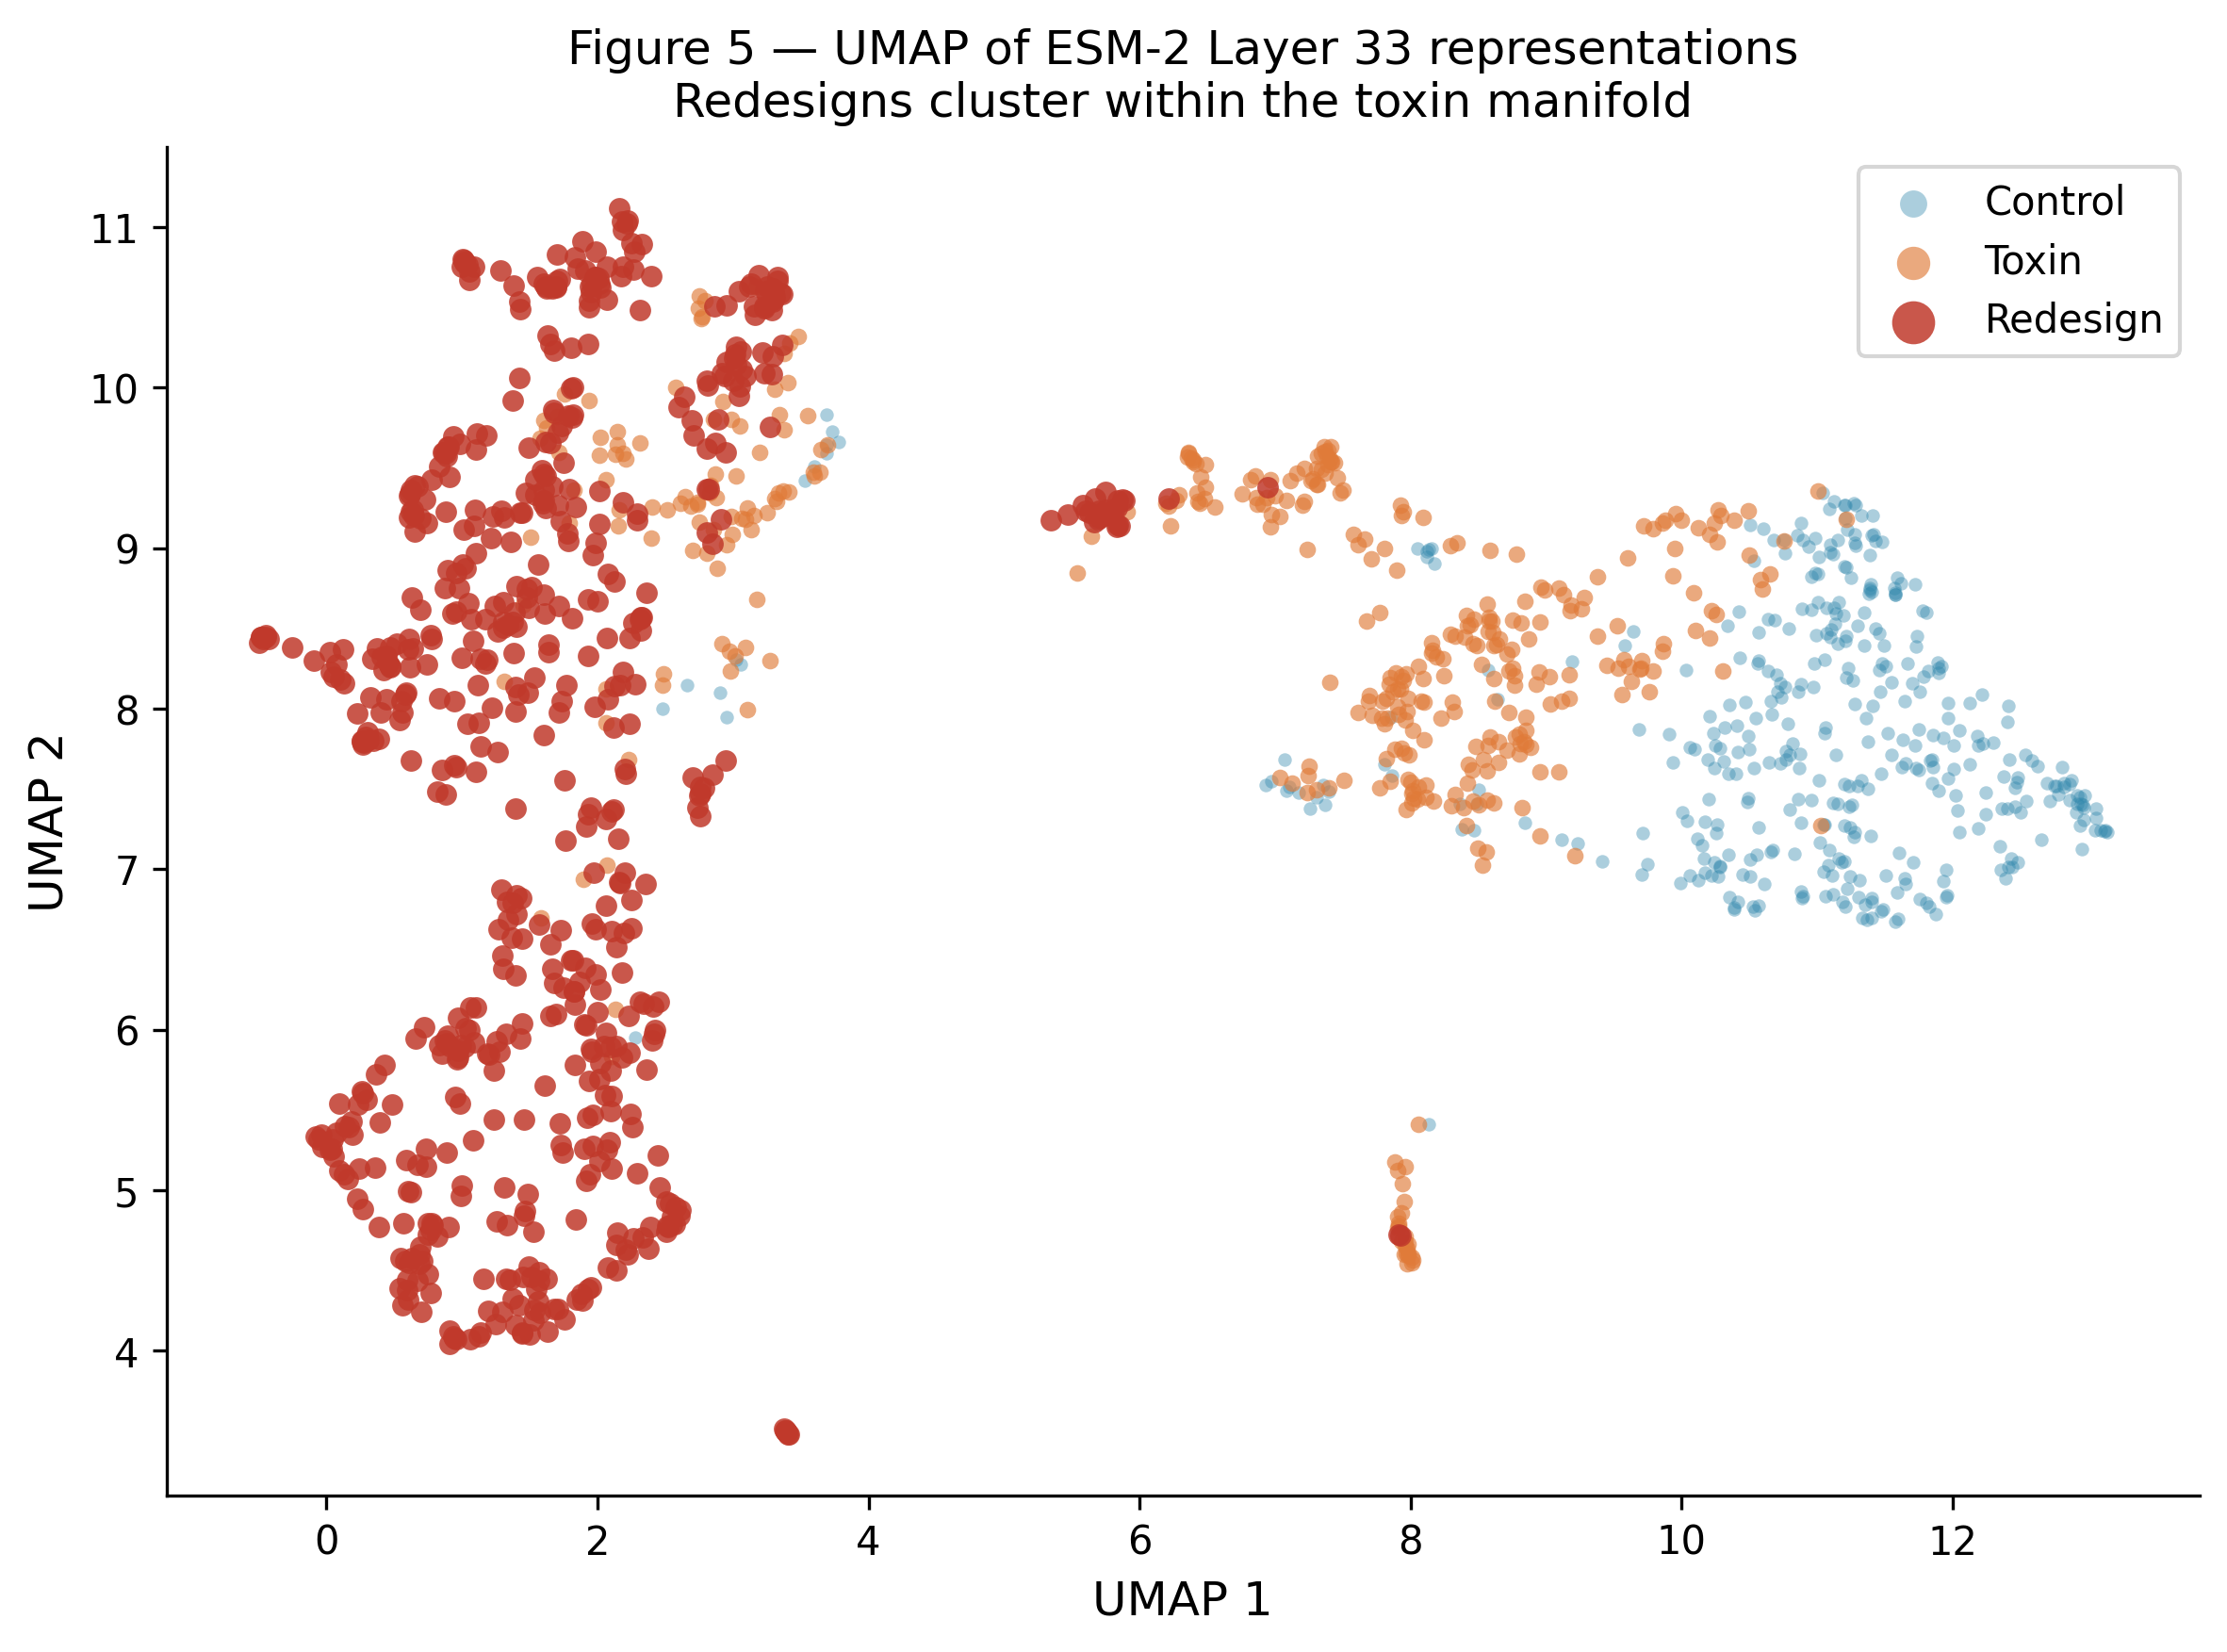
\includegraphics[width=0.8\textwidth]{figures/fig5_umap.png}
\caption{UMAP projection of ESM-2 embeddings. Redesigns (red) cluster with natural toxins (orange), not controls (blue).}
\end{figure}


\textbf{Representational Similarity Analysis (RSA):}

\begin{table}[H]
\centering
\begin{tabular}{lc}
\toprule
\textbf{Comparison} & \textbf{Mean cosine distance} \\
\midrule
Toxin $\leftrightarrow$ Toxin & 0.0680 \\
Toxin $\leftrightarrow$ Redesign & 0.0647 \\
Toxin $\leftrightarrow$ Control & 0.1400 \\
Redesign $\leftrightarrow$ Control & 0.1453 \\
\midrule
Class separability & \textbf{2.16$\times$} \\
RSA Spearman $r$ & $-0.007$ ($p = 0.648$) \\
\bottomrule
\end{tabular}
\caption{Redesigns are 2.16$\times$ closer to toxins than to controls (0.065 vs 0.145), confirming ProteinMPNN preserves the toxin neighbourhood. However, internal pairwise geometry is not preserved (RSA $r = -0.007$)---ProteinMPNN scrambles relative positions while maintaining the class boundary.}
\end{table}

% ============================================================
\section{Discussion}
% ============================================================

\subsection{Why ProteinMPNN Fails to Evade ESM-2}

ProteinMPNN optimises sequence identity reduction while preserving protein backbone geometry.
Structure is precisely what ESM-2's toxin circuit encodes. The transfer ratio of 1.28
is not merely ``the probe still works''---it is evidence that ProteinMPNN redesign
\textit{amplifies} the structural motifs that make toxins detectable. Redesigns are 2.16$\times$
closer to natural toxins than to controls in ESM-2 embedding space (RSA separability = 2.16),
and the circuit correlation $r = 0.992$ confirms they activate the same representational pathway.

\subsection{The Circuit Architecture}

\begin{enumerate}
    \item \textbf{Early layers (1--9)}: Sequence-level features (AUROC 0.97 by L9)
    \item \textbf{Mid layers (17--20)}: Primary toxin discrimination (DPA +40--45)
    \item \textbf{Suppressor layers (27--28)}: Internal regulation
    \item \textbf{Final layers (29--32)}: Strong final-phase discrimination (DPA +23--130), with layer 32 as primary bottleneck
    \item \textbf{Multiple pathways}: ProteinMPNN redesigns achieve the same endpoint via only 19\% circuit overlap with natural toxins---ESM-2 has multiple routes to the toxin representation, making targeted disruption difficult
\end{enumerate}

\subsection{The Security Boundary}

The four-tier attack taxonomy reveals the security boundary lies at gradient access:

\begin{itemize}
    \item \textbf{No gradient + structural constraint (ProteinMPNN)}: 6.1\% evasion. Practical threat model---produces functional proteins via synthesis orders.
    \item \textbf{Gradient + no structural constraint (HotFlip)}: 100\% evasion. Requires white-box probe access; unconstrained substitutions may compromise protein function (to be confirmed by structural prediction).
    \item \textbf{Embedding-space attacks (PGD, pSSR/UAP)}: 100\% evasion. Require white-box access to ESM-2 internals; no sequence-space realisation without embedding inversion.
\end{itemize}

The UAP's stable attack geometry (cos $= -0.805$ invariant to $\epsilon$) reveals why:
the robust SAE features that bind all toxins together in embedding space (making them
resistant to sequence attack) simultaneously create a thin manifold that one gradient-optimised
vector can cross universally. \textbf{The probe's security guarantee is exactly as strong as
the privacy of its weights.}

\subsection{Biosecurity Implications}

\begin{enumerate}
    \item \textbf{Sequence-based screening is insufficient}: All 723 redesigns evade BLAST.
    \item \textbf{ESM-2 probes are robust by architecture}: Transfer ratio 1.28 means the adversary is working against themselves---ProteinMPNN preserves what the probe detects.
    \item \textbf{No retraining needed}: 93.9\% detection with zero exposure to redesigned sequences; cross-family holdout AUROC 0.9929 confirms generalisation to unseen toxin families.
    \item \textbf{Zero-shot discovery}: The probe finds biosecurity threats not in any training set, including a WHO Priority 1 pathogen cluster and cross-kingdom fungal effectors---functioning as an open-ended discovery tool, not just a known-threat detector.
    \item \textbf{Deployment recommendation}: Deploy ESM-2 probes with private weights. The security margin at $\epsilon = 0.5$ in embedding space is not practically reachable by synthesis-order adversaries without model internals.
    \item \textbf{Interpretability enables targeted hardening}: The evadable features (transfer ratio ${<}0.13$) represent known blind spots. A screening system could flag anomalous patterns where robust features fire but evadable features do not---consistent with targeted evasion.
\end{enumerate}

\subsection{Limitations}

\begin{itemize}
    \item \textbf{HotFlip functional validation}: Whether HotFlip sequences retain toxin function is unconfirmed; structural constraints differ from ProteinMPNN's explicit backbone preservation.
    \item \textbf{DMS single sequence}: The N29 polarity-not-identity finding is demonstrated on one representative toxin; generalisation across families requires additional DMS experiments.
    \item \textbf{Wet-lab validation}: Computational predictions require experimental confirmation, particularly the two uncharacterised \textit{A. baumannii} candidates (0.9995, 0.9993).
    \item \textbf{Single redesign tool}: Extension to EvoDiff and RFdiffusion is ongoing.
    \item \textbf{Embedding inversion}: Embedding-space attacks do not directly produce sequences; the gap between embedding-space and sequence-space evasion quantifies the inversion cost.
\end{itemize}

% ============================================================
\section{Open Problems (Future Work)}
% ============================================================

\begin{enumerate}
    \item \textbf{HotFlip transferability}: Do gradient-guided sequence attacks transfer across probe architectures and pLMs, analogous to GCG transferability across LLMs \cite{zou2023universal}? If so, probe diversity alone does not provide security.
    
    \item \textbf{Protein alignment}: ProteinMPNN has no alignment objective---it will design dangerous proteins given the right backbone. Fine-tuning protein design models using circuit-level interventions at the layer-32 bottleneck (the protein-space analogue of RLHF) could make design models intrinsically safer rather than relying on output filters.
    
    \item \textbf{Wet-lab validation}: AlphaFold structural prediction of the two uncharacterised \textit{A. baumannii} candidates (UniRef50\_A0A009RXF9, UniRef50\_A0A009QBX0) followed by cytotoxicity assays would transform a computational prediction into a biosecurity discovery. Collaboration with IBBIS/CBH is the natural path.
    
    \item \textbf{Attack taxonomy across pLMs}: A systematic benchmark of (pLM $\times$ probe architecture $\times$ attack type) would establish principled deployment recommendations---the protein-space analogue of AdvBench.
\end{enumerate}

% ============================================================
\section{Conclusions}
% ============================================================

\begin{itemize}
    \item \textbf{BLAST: 0\%. ESM-2: 93.9\%.} ProteinMPNN fails to evade structure-aware probes.
    \item \textbf{Transfer ratio 1.28}: Redesigns amplify toxin features---ProteinMPNN preserves what the probe detects.
    \item \textbf{r = 0.992}: Redesigns use the same DPA circuit as natural toxins; 19\% circuit overlap means multiple routes to the same toxic endpoint.
    \item \textbf{Security boundary at gradient access}: 6.1\% evasion (blackbox) vs 100\% (white-box gradient). The probe's guarantee equals the privacy of its weights.
    \item \textbf{UAP geometry}: Stable attack direction (cos $= -0.805$, invariant to $\epsilon$) reveals manifold structure, not probe weakness.
    \item \textbf{Zero-shot discovery}: Hemolysin, Leukotoxin, Cyclolysin, fungal effector Ecp2, and two uncharacterised \textit{A. baumannii} proteins---none in training data.
    \item \textbf{Mutation robustness}: 0/1,179 single-point mutations evade; the circuit reads polarity, not sequence identity.
\end{itemize}

\textbf{The key insight}: ProteinMPNN cannot redesign away what is structurally necessary for toxin function---and ESM-2 reads structure.

\subsection*{Software Artifacts}
\begin{enumerate}
    \item \textbf{\texttt{screen.py}}: Zero-shot CLI screening tool with layer-wise DPA attribution.
    \item \textbf{\texttt{demo.ipynb}}: Interactive notebook for screening and visualisation.
\end{enumerate}

% ============================================================
\section*{Key Numbers Reference}
% ============================================================
\begin{table}[H]
\centering
\begin{tabular}{lc}
\toprule
\textbf{Metric} & \textbf{Value} \\
\midrule
Training toxins & 1,712 \\
Training controls & 2,072 \\
ProteinMPNN redesigns & 723 \\
Best probe layer & 33 \\
Probe AUROC (natural test) & 0.9970 \\
BLAST detection on redesigns & \textbf{0.0\%} \\
ESM-2 detection on redesigns & \textbf{93.9\%} \\
Double-Evaders (BLAST + Probe evasion) & 92 \\
SAE True Recovery of Double-Evaders & \textbf{38\%} (35/92) \\
Mean transfer ratio & \textbf{1.28} \\
Cross-family holdout AUROC & \textbf{0.9929} \\
SAE features total & 10,240 \\
Dead SAE features & 8,345 (81.5\%) \\
Top-K features used & 50 \\
Compression ratio & 205$\times$ \\
SAE AUROC (top-50) & 0.9447 \\
DPA tox/redesign correlation & \textbf{$r = 0.992$} \\
Circuit overlap (nat vs redesign) & 19\% \\
RSA class separability & 2.16$\times$ \\
Steering ($\alpha = 2.0$, controls) & $0.000 \rightarrow 1.000$ \\
UAP security margin & $\epsilon = 0.5$ \\
UAP cos (stable across all $\epsilon$) & $-0.805$ \\
DMS single-point evasion & 0/1,179 \\
UniRef50 candidates & 248 / 1,000 \\
Signal peptide enrichment & 4.75$\times$ ($p < 0.001$) \\
ProteinMPNN evasion & \textbf{6.1\%} \\
HotFlip evasion & 100\%$^\dagger$ \\
PGD evasion & 100\% \\
pSSR evasion & 100\% \\
\bottomrule
\end{tabular}
\end{table}

\noindent $^\dagger$HotFlip sequences may not retain protein function; wet-lab validation pending.

\begin{thebibliography}{9}
\bibitem{wittmann2025}
Wittmann, B.J., et al. (2025). Strengthening nucleic acid biosecurity screening against generative protein design tools. \textit{Science}.

\bibitem{zou2023universal}
Zou, A., et al. (2023). Universal and Transferable Adversarial Attacks on Aligned Language Models. \textit{arXiv:2307.15043}.

\bibitem{madry2018pgd}
Madry, A., et al. (2018). Towards Deep Learning Models Resistant to Adversarial Attacks. \textit{ICLR 2018}.

\bibitem{simon2024interplm}
Simon, E., \& Zou, J. (2024). Discovering Interpretable Features in Protein Language Models via Sparse Autoencoders. \textit{bioRxiv}.

\bibitem{adams2025saeplm}
Adams, R., et al. (2025). From Mechanistic Interpretability to Mechanistic Biology. \textit{bioRxiv}.
\end{thebibliography}

\end{document}
